\documentclass[a4paper,10pt]{book}
\usepackage[T1]{fontenc}
\usepackage[latin9]{inputenc}
\usepackage{amsmath}
\usepackage{amssymb}
\usepackage{listings}
\usepackage{enumerate}
\usepackage{enumitem}
\usepackage{multirow}
\usepackage[colorlinks = true,
            linkcolor = blue,
            urlcolor  = blue,
            citecolor = blue,
            anchorcolor = blue]{hyperref}
\usepackage{makecell}
\usepackage{pifont}
\usepackage{float}
\usepackage{listings}
\usepackage{tikz}
\usepackage{nicematrix}


\newcommand\when{\  when\ }
\newcommand\otherwise{\  otherwise\ }

\newcommand\doubleplus{+\kern-1.3ex+\kern0.8ex}
\newcommand\mdoubleplus{\ensuremath{\mathbin{+\mkern-10mu+}}}

\newcommand{\false}{f\kern-0.25ex{alse}}
\newcommand\mfalse{\ensuremath{\mathbin{f\mkern-5mu alse}}}

\newcommand\f{\textit{f}}


 

\lstset{emph={Int,count,abs,repeating,Array}, emphstyle=\color{itemcolor}}


\makeatletter
\newcommand{\skipitems}[1]{%
  \addtocounter{\@enumctr}{#1}%
}


\title{Functional Levitin}
\author{Lee Barney}

\begin{document}
\maketitle
\date{\today}
\frontmatter
\chapter{Prologue}
Levitin is a good book to use when learning how to analyze and improve algorithms. It does, however, have one big drawback when using a functional approach. The example and problem algorithms presented do not use a functional-style pseudocode. This booklet intends to translate all of Levitin's algorithms presented into functional style using a functional pseudocode.

This booklet is designed so that its chapters and chapter sub-sections match the numbering of Levitin's book. At times, parameter pattern matching is used when describing the algorithms. At other times, guards are used. Our choice of which to use is usually determined by which choice makes the algorithm clearer. Sometimes, we choose one that makes the algorithm a little less clear. This is usually done for educational reasons.

We have also taken the liberty to rename some of the algorithms. We prefer algorithm names that are verbs. After all, algorithms do things and verbs do things.

Also, the pseudocode followed in this document follows that described in this \href{https://byui-cse.github.io/cse382-course/pseudocode_primer.html}{documentation and primer document}.

Enjoy!
\chapter{Things to Know}

Here are a few algorithms Levitin doesn't include in his book that every person doing Functional Design needs to know, not just be aware of. Without these, life becomes very hard.

\section{Map}
Time Complexity: $\mathcal{O}(n)$

\begin{align*}
map\ ::\ &[a](\lambda::a\rightarrow b)\rightarrow[b]\\
map\ ::\ &[]\ \_\rightarrow []\\
map\ ::\ &[h\mid t]\  \lambda\rightarrow\\
&[\lambda\ h]\doubleplus(map\ t\ \lambda).
\end{align*}
\section{Filter}
Time Complexity: $\mathcal{O}(n)$

\subsection{Using Parameter Pattern Matching}

\begin{align*}
filter\ ::\ &[a](\lambda::a\rightarrow b:::Boolean)\rightarrow[a]\\
filter\ ::\ &[]\ \_\rightarrow []\\
filter\ ::\ &[h\mid t]\  \lambda\rightarrow\\
&\quad case\ \lambda\ h\\
&\quad\quad true\rightarrow [h]\doubleplus(filter\ t\ \lambda)\\
&\quad\quad\false\rightarrow filter\ t\ \lambda.
\end{align*}

\subsection{Using Guards}
\begin{align*}
  filter &:: [a]\ (\lambda :: a\rightarrow Boolean)\rightarrow[b]\\
  filter &:: [a]\ (\lambda :: a\rightarrow Boolean)\rightarrow [\ ]\ \ when\ [a]\text{ is empty };\\
  filter &:: [h\mid t]\ (\lambda :: a\rightarrow Boolean)\rightarrow\\
  &[h]\doubleplus filter\ t\ \lambda\ 
  when\ \lambda\ h = true\\
  &filter\ t\ \lambda\ 
  otherwise.
  \end{align*}
  
 \section{Fold Left} 
Time Complexity: $\mathcal{O}(n)$

Create a single solution from a list starting from the left and going to the right. Also known as 'reduce'.
\begin{align*}
\f old\_l\ ::\ &[a](\lambda::a\ acc\rightarrow b)\ acc\rightarrow[b]\\
\\
\f old\_l\ ::\ &[]\ \_\ acc\rightarrow acc\\
\f old\_l\ ::\ &[h\mid t]\  \lambda\ acc\rightarrow\\
&\f old\_l\ t\ \lambda\ (\lambda\ h\ acc).
\end{align*}

\mainmatter
\chapter{Introduction}
\section{What is an Algorithm?}
\subsection{Euclid's GCD algorithm}
Time Complexity: $\mathcal{O}(\log n)$

\begin{align*}
gcd\ ::\ &a\ a\rightarrow a:::Integer \ge 0\\
gcd\ ::\ &m\ 0\rightarrow m\\
gcd\ ::\ &m\ n\rightarrow gcd\ n\ (m\mod n)
\end{align*}

\subsection{Sieve of Eratosthenese}

Time Complexity: $\mathcal{O}(n^2)$

Here is a naive version of this algorithm.
Its data consists of an accumulator, used to gather the primes, and a sequence of integers 2 through some number of interest in which primes are to be discovered. A helper function, $is\_multiple\_of$ is used to increase readability.
\begin{align*}
sieve\ ::\ &acc\ [2\ldots a]\rightarrow [a]\\
sieve\ ::\ &acc\ []\rightarrow acc\\
sieve\ ::\ &acc\ [h\mid t]\rightarrow\\
	&\quad case\ is\_multiple\_of\ acc\ h\\
	&\quad\quad true\rightarrow sieve\ acc\ t\\
	&\quad\quad false\rightarrow sieve\ h\doubleplus acc\ t
\end{align*}
\subsubsection{Sub-Algorithm}
Time Complexity: $\mathcal{O}(n)$

\begin{align*}
is\_multiple\_of\ ::\ &[a:::Integer] a\rightarrow Boolean\\
is\_multiple\_of\ ::\ &[]\ a\rightarrow false\\
is\_multiple\_of\ ::\ &[h\mid t]\ a\rightarrow\\
	&\quad case\ 0\equiv a\pmod h\\
	&\quad\quad true\rightarrow true\\
	&\quad\quad false\rightarrow is\_multiple\_of\ t\ a
\end{align*}
\section{Fundamentals of Algorithmic Problem Solving}
None.
\section{Important Problem Types}
None.
\section{Fundamental Data Structures}
None.
\chapter{Fundamentals of the Analysis of Algorithm
Efficiency}
\section{The Analysis Framework}
\subsection{Sequential Search}
Time Complexity: $\mathcal{O}(n)$

This sequential search algorithm is a variation of the maximum element algorithm.
\begin{align*}
seq\_search\ ::\ &[a]\ [a]\ a\rightarrow b\\
seq\_search\ ::\ &[]\_\ \_\rightarrow -1;\\
seq\_search\ ::\ &[h|t]\ key\ location\rightarrow\\
& location\ when\ h=key\\
&seq\_search\ t\ key\ location+1\ otherwise.
\end{align*}

\section{Asymptotic Notations and Basic Efficiency Classes}
There are no algorithms described by Levitin in this part of the reading.

\section{Mathematical Analysis of Nonrecursive Algorithms}

\subsection{Maximum Element}
This algorithm is used to find the maximum element in an unordered list. The elements are all comparable using the comparison function $\lambda\ ::\ a\ a\rightarrow r:::Integer$ that has as parameters two items comparable using the instance of the $\lambda$ function, and has a value that is $-1$ if the right parameter is less than the left parameter, $1$ if the right parameter is greater than the left parameter, and $0$ if they are equal.  
\begin{align*}
find\_max\_element\ ::\ &[a]\ a\ \lambda\rightarrow a\\
find\_max\_element\ ::\ &[]\ accum\ \_\rightarrow accum;\\
find\_max\_element\ ::\ &[h\mid t]\ accum\ \lambda\ when\ (\lambda\ h\ accum) = 1\rightarrow\\
	&find\_max\_element t h;\\
find\_max\_element\ ::\ &[\_\mid t]\ accum\ \_ otherwise\rightarrow\\
	&find\_max\_element\ t\ accum.
\end{align*}

\subsection{All Elements are Unique}
Time Complexity: $\mathcal{O}(n^2)$

This algorithm determines if each element of the list is unique. If this is so, the algorithm has a value of $true$, otherwise its value is $false$. It also uses a helper algorithm, $compare\_to\_all$, to increase readability.

\begin{align*}
is\_fully\_unique\ ::\ &[a]\ [a]\rightarrow Boolean\\
is\_fully\_unique\ ::\ &[]\ \_\rightarrow true;\\
is\_fully\_unique\ ::\ &[h\mid t]\ checked\rightarrow\\
	&case\ is\_found\_in\ h\ (checked\doubleplus t)=true\\
	&\quad true\rightarrow\false\ \\
	&\quad is\_fully\_unique\ t\ h\doubleplus checked\ otherwise.
\end{align*}
\subsubsection{Uniqueness Helper Function}
Time Complexity: $\mathcal{O}(n)$
\begin{align*}
is\_found\_in\ ::\ &[a]\ a\rightarrow Boolean\\
is\_found\_in\ ::\ &[]\ \_\rightarrow \false;\\
is\_found\_in\ ::\ &[h\mid t]\ a\rightarrow\\
	&true\ when\ h=a\\
	&\false\ otherwise
\end{align*}
\subsection{Matrix Multiplication}
Levitin's \textit{MatrixMultiplication} algorithm is broken up here and presented in smaller pieces that combine to make bigger pieces. While the first algorithms shown here are used by the \textit{multiply} algorithm below, they are not sub-algorithms as they are frequently used independently of doing matrix multiplication.

\subsubsection{Vector Scalar Product}
Time Complexity: $\mathcal{O}(n)$

\begin{align*}
vector\_scalar\ ::\ &a\ [a]\ accum\rightarrow a\\
vector\_scalar\ ::\ &\_\ []\ accum\rightarrow accum;\\
vector\_scalar\ ::\ &a\ [h\mid t]\ accum\rightarrow\\
	&vector\_scalar\ a\ t\ (accum+a\cdot h).
\end{align*}

\subsubsection{Vector Dot Product}
Time Complexity: $\mathcal{O}(n)$

This algorithm has as its value a Real that is the dot product of two equal-lengthed Vectors with Real elements.
\begin{align*}
vector\_dot\ ::\ &[a]\ [a]\ a\ \rightarrow a:::Real\\
vector\_dot\ ::\ &[]\ \_\ accum\rightarrow accum;\\
vector\_dot\ ::\ &[h\mid t]\ [hn\mid tn]\ accum\rightarrow\\
	&vector\_dot\ t\ tn\ accum+h\cdot hn.
\end{align*}

\subsubsection{Matrix Multiplication}
Time Complexity: $\mathcal{O}(n^3)$

This naive algorithm multiplies two square matrices of Reals of equal dimensions. The first matrix is represented as a list of rows. The second matrix is represented as a list of columns. Each row and column is also a list. This algorithm uses the $build\_row\_using$ helper algorithm for ease of reading.

\begin{align*}
multiply\ ::\ &[[a]]\ [[a]]\rightarrow [[a:::Real]]\\
multiply\ ::\ &[]\ \_\rightarrow accum;\\
multiply\ ::\ &[h\mid t]\ columns\rightarrow\\
	&(build\_row\_with\ h\ columns)\doubleplus multiply\ t\ columns.
\end{align*}
\subsubsection{Sub-Algorithm}
Time Complexity: $\mathcal{O}(n^2)$

The value of this helper algorithm is a row of calculated values.
\begin{align*}
build\_row\_using\ ::\ &[a]\ [a]\rightarrow [a]\\
build\_row\_using\ ::\ &\_\ []\rightarrow [];\\
build\_row\_using\ ::\ &r\ [h\mid t]\rightarrow\\
&[vector\_dot\ r\ h]\doubleplus build\_row\_using\ r\ t.
\end{align*}

\subsubsection{Binary Digit Counter}Time Complexity: $\mathcal{O}(n)$ where $n$ is the number of binary digits required to represent the base 10 number passed as parameter 1.

\begin{align*}
count\_binary\_digits\ ::\ &a\ a\rightarrow a:::Integer\\
count\_binary\_digits\ ::\ &1\ accum\rightarrow accum;\\
count\_binary\_digits\ ::\ &a\ accum\rightarrow\\
	&count\_binary\_digits\ \lfloor a\div 2 \rfloor\ accum+1.
\end{align*}

\subsubsection{Mystery Algorithm, 2.3 \#4}

When $mystery$ is used, $a$ must always be greater than 0 and $accum$ is initialized to $0$.
\begin{align*}
mystery\ ::\ &a\ a\rightarrow a:::Integer\\
mystery\ ::\ &0\ accum\rightarrow accum;\\
mystery\ ::\ &a\ accum\rightarrow accum+ a\cdot a.
\end{align*}

\subsubsection{Secret Algorithm, 2.3 \#5}

When $secret$ is used, $max\_accum$ is initialized to $-\infty$ and $min\_accum$ is initialized to $\infty$.
\begin{align*}
secret\ ::\ &[a]\ a\ a\rightarrow a:::\{Real,Real\}\\
secret\ ::\ &[]\ max\_accum\ min\_accum\rightarrow \{max\_accum,min\_accum\};\\
secret\ ::\ &a\ accum\rightarrow accum+ a\cdot a.
\end{align*}

\subsubsection{Gausian Elimination, 2.3 \#10}

\begin{align*}
TO DO
\end{align*}
\section{Mathematical Analysis of Recursive Algorithms}

\subsubsection{Factorial}
Time Complexity: $\mathcal{O}(n)$. Space Complexity: $\mathcal{O}(n^2)$ for data being a natural number.
\begin{align*}
factorial ::\ &a\rightarrow a:::Integer\ge 0\\
factorial ::\ &0 \rightarrow 1;\\
factorial ::\ &a\rightarrow\\
       &\quad a\cdot factorial ::\ a-1.
\end{align*}

\subsubsection{Sum $n$ Cubes, 2.4 \#3}

\begin{align*}
sum\_cubes\ ::\ &a\rightarrow a:::Integer\ge 0\\
sum\_cubes\ ::\ &1\rightarrow 1;\\
sum\_cubes\ ::\ &a\rightarrow\\
	&a\cdot a\cdot a+sum\_cubes\ a-1.
\end{align*}

\subsubsection{Q, 2.4 \#4}

\begin{align*}
q\ ::\ &a\rightarrow a:::Integer\ge 0\\
q\ ::\ &1\rightarrow 1;\\
q\ ::\ &a\rightarrow\\
	&2\cdot a-1+(q\ a-1).
\end{align*}

\subsubsection{Riddle, 2.4 \#9}

\begin{align*}
riddle\ ::\ &[a]\rightarrow a:::Real\ge 0\\
riddle\ ::\ &[]\rightarrow \infty;\\
riddle\ ::\ &[h\mid t]\rightarrow\\
	&temp\leftarrow riddle\ t,\\
	&case temp\le h\\
	&\quad true\rightarrow temp\\
	&\quad\false\rightarrow h.
\end{align*}
2.4 \#9 part c: Rewrite this algorithm so it is tail-recursive. Does this change your answer for part b? Why or why not?

\subsubsection{Graph Complete, 2.4 \#10}

\begin{align*}
graph\_complete\ ::\ &[[a:::Integer]]\rightarrow Boolean\\
graph\_complete\ ::\ &[]\rightarrow true;\\
graph\_complete\ ::\ &[h\mid t]\rightarrow\\
	&case vector\_complete h\\
	&\quad\false\rightarrow false\\
	&\quad true\rightarrow graph\_complete\ t.
\end{align*}

(Sub-Algorithm) Time Complexity: best case $\mathcal{O}(1)$, average and worst case $\mathcal{O}(n)$.
\begin{align*}
vector\_complete\ ::\ &[a:::Integer]\rightarrow Boolean\\
vector\_complete\ ::\ &[]\rightarrow true;\\
vector\_complete\ ::\ &[h\mid \_]\ when\ h=0\rightarrow false;\\
vector\_complete\ ::\ &[\_\mid t]\ otherwise\rightarrow\\
	&vector\_complete\ t.
\end{align*}

\section{Example: Computing the n\textsuperscript{th} Fibonacci Number}

\subsection{$n^{th}$ Fibonacci Number Generation}

\begin{align*}
gen\_fib\ ::\ &a\rightarrow a:::Integer\\
gen\_fib\ ::\ &0\rightarrow 0;\\
gen\_fib\ ::\ &a\rightarrow (gen\_fib\ n-1) + (gen\_fib\ n-2)
\end{align*}

\section{Empirical Analysis of Algorithms}
\subsection{Pseudorandom Numbers}

When this linear congruential method algorithm is used, the $r$ parameter is the seed and $m$ is used as $modulo$. Change the seed and you get a different set of random numbers in $(0,1)$.
\begin{align*}
random\ ::\ &a\ a\ a\ a\ a\rightarrow [a:::Integer]\\
random\ ::\ &0\ \_\ \_\ \_\ \_\rightarrow [];\\
random\ ::\ &count\ m\ r\ multiplier\ addend\rightarrow \\
&rand\_digit\leftarrow a\cdot r+b\pmod{m}\\
&[rand\_digit]\doubleplus random\ count-1\ m\ rand\_num\ multiplier.
\end{align*}

\subsection{Sort Analysis, 2.6 \#1}
\begin{align*}
analyze\_sorting\ ::\ &[a]\ [a]\rightarrow [a]\\
analyze\_sorting\ ::\ &[]\ accum\rightarrow accum;\\
analyze\_sorting\ ::\ &[h\mid t]\ accum\rightarrow \\
	&analyze\_sorting\ ::\ &t\ insert\_into\ accum\ h.
\end{align*}

\subsubsection{Sub-Algorithm}
\begin{align*}
insert\_into\ ::\ &[a]\ a\rightarrow [a]\\
insert\_into\ ::\ &[]\ a\rightarrow [a];\\
insert\_into\ ::\ &[h\mid t]\ a\ when\ h>a\rightarrow\\
	&[h]\doubleplus\ insert\_into\ t\ a;\\
insert\_into\ ::\ &[h\mid t]\ a\ otherwise\rightarrow\\
	&[a]\doubleplus[h]\doubleplus t.
\end{align*}
Modify this algorithm so that it accurately counts, and has as its value, how many times a comparison was executed.
 
\chapter{Brute Force and Exhaustive Search}
\section{Selection Sort and Bubble Sort}
\subsection{Selection Sort}
Time Complexity: $\mathcal{O}(n^2)$

This algorithm uses the $pick$ sub-algorithm.
\begin{align*}
sel\_sort\ ::\ &[a]\ [a]\rightarrow[a]\\
sel\_sort\ ::\ &[]\ acc\rightarrow acc;\\
sel\_sort\ ::\ &[h|t]\ acc\rightarrow\\
       &\quad \{selected,remaining\}\leftarrow pick\ t\ h\ []\\
&\quad sel\_sort\ ::\ t\ selected\doubleplus acc.
\end{align*}
\subsubsection{Sub-Algorithm}Time Complexity: $\mathcal{O}(n)$
\begin{align*}
pick\ ::\ &[a]\ a\ [a]\rightarrow\{a,[a]\}\\
pick\ ::\ &[]\ picked\ acc\rightarrow\\
 &\{picked,acc\};\\
pick\ ::\ &[h|t]\ picked\ acc\rightarrow\\
       &\quad case\ h>picked\\
&\quad\quad  true\rightarrow\\
&\quad\quad\quad\ pick\ ::\ t\ h\ acc\doubleplus picked\\
&\quad\quad\false\rightarrow\\
&\quad\quad\quad pick\ t\ picked\ acc\doubleplus h;
\end{align*}

\subsection{Bubble Sort}Time Complexity: $\mathcal{O}(n^2)$

This Bubble Sort description has a list sorted least to greatest as its value. It uses the $density\_move$ sub-algorithm found below.
\begin{align*}
b\_sort\ ::\ &[a]\ [a]\rightarrow [a]\\
b\_sort\ ::\ &[]\ accum\rightarrow accum;\\
b\_sort\ ::\ &[h\mid t]\ accum\rightarrow\\
	&\{greatest, lesser\}\leftarrow density\_move\ t\ h,\\
	&b\_sort\ lesser\ greatest\doubleplus accum.
\end{align*}

\subsubsection{Sub-Algorithm}Time Complexity: $\mathcal{O}(n)$

This algorithm moves each element in a list towards the end based on its density. Here, density is loosely defined as 'greater-than' for what ever the type is for the elements in the list. The most dense element is removed from the list and the less dense elements are accumulated in, potentially, shifted positions.
 
\begin{align*}
density\_move\ ::\ &[a]\ [a]\ a\rightarrow \{a,[a]\}\\
density\_move\ ::\ &[]\ accum\ most\_dense\rightarrow \{most\_dense,accum\};\\
density\_move\ ::\ &[h\mid t]\ accum\ current\ when\ h\ge current\rightarrow\\
	&density\_move\ t\ ( accum\doubleplus [current])\ h;\\
density\_move\ ::\ &[h\mid t]\ accum\ current\ otherwise\rightarrow\\
	&density\_move\ t\ (accum\doubleplus[h])\ current.
\end{align*}
\section{Sequential Search and Brute-Force String Matching}
\subsection{Sequential Search}
Time Complexity: $\mathcal{O}(n)$

This sequential search algorithm is a variation of the maximum element algorithm. This algorithm has a 1-based location as its value rather than a 0-based index. A value of $-1$ indicates the key was not found in the list.
\begin{align*}
seq\_search\ ::\ &[a]\ [a]\ a\rightarrow b\\
seq\_search\ ::\ &[]\_\ \_\rightarrow -1;\\
seq\_search\ ::\ &[h\mid \_]\ key\ when\ h=key\rightarrow 1;\\
seq\_search\ ::\ &[\_\mid t]\ key\ otherwise\rightarrow\\
	&1+seq\_search\ t\ key.
\end{align*}

\section{Brute Force String Matching}Time Complexity: $\mathcal{O}(nm)$ for $m$ being the length of the text to be searched, and $n$ being the length of the text being searched for.

This naive algorithm searches for a specific string within a text string and returns the 1-based location, not the 0-based index, of the beginning of the first instance of the search string if it is found, and $-1$ if not. To accomplish this, it uses the $starts\_with$ sub-algorithm.
\begin{align*}
bf\_string\_match\ ::\ &[c]\ [c:::Character]\rightarrow Integer\\
bf\_string\_match\ ::\ &\_\ []\rightarrow -1;\\
bf\_string\_match\ ::\ &search\_string\ text\_string\rightarrow\\
	&\quad case\ starts\_with\ search\_string\ text\_string\\
&\quad  true\rightarrow\\
&\qquad\quad 1\\
&\quad\false\rightarrow\\
&\qquad\quad [h\mid t]\leftarrow text\_string\\
&\qquad\quad 1+bf\_string\_match\ search\_string\ t;
\end{align*}
\subsection{Sub-Algorithm}Time Complexity: $\mathcal{O}(n)$
\begin{align*}
starts\_with\ ::\ &[c]\ [c:::Character]\rightarrow Boolean\\
starts\_with\ ::\ &[]\_\rightarrow true;\\
starts\_with\ ::\ &[sh\mid st]\ [th\mid tt]\when sh\ne th\rightarrow\false;\\
starts\_with\ ::\ &[sh\mid st]\ [th\mid tt]\otherwise\rightarrow\\
&starts\_with\ st\ tt;
\end{align*}

\section{Brute Force Closest Pair}Time Complexity: $\mathcal{O}(n^2)$.

The description of this algorithm doesn't declare a specific type for the elements of the list, other than the types are in a tuple. The type could be anything that is comparable and for which differences can be calculated. For example, real numbers, integers, strings, people, dogs, cats, stars, etc. Use your imagination. 

Two $\lambda$s, comparator and difference, are used that allow this abstraction to work. Each of these $\lambda$s has two parameters of the type in the list. A further abstraction, not included in this algorithm, would be abstracting away the use of list. The complexity declaration for this algorithm assumes the time complexity class of both $\lambda$s is $\mathcal{O}(1)$.

This algorithm uses the sub-algorithm $\text{\textit{find}}\_closest\_to$.

\begin{align*}
bf\_closest\_pair\ ::\ &[a]\ \{a,a\}\ \lambda\ \lambda\ \rightarrow \{a,a\}\\
bf\_closest\_pair\ ::\ &[]\ accum\ \_\ \_\ \rightarrow accum\\ 
bf\_closest\_pair\ ::\ &[h\mid t]\ \{a_1,a_2\}\ comparator\ \text{\textit{difference}}\ \rightarrow\\
	&closest\leftarrow \text{\textit{find}}\_closest\_to\ h\ t\ a_1\ comparator,\\
	&case\ \big | \text{\textit{difference}}\ h\ closest\big |<\big |\text{\textit{difference}}\ a_1,a_2\big |\\
	&\quad true\\
	&\qquad bf\_closest\_pair\ t\ \{h,closest\}\ comparator\ \text{\textit{difference}}\\
	&\quad\false\\
	&\qquad bf\_closest\_pair\ t\ \{a_1,a_2\}\ comparator\ \text{\textit{difference}}.\\ 
\end{align*}
\subsection{Sub-Algorithm}

\begin{align*}
\text{\textit{find}}\_closest\_to\ ::\ &a\ [a]\ a\ \lambda\rightarrow a\\
\text{\textit{find}}\_closest\_to\ ::\ &\_\ []\ accum\ \_\rightarrow accum\\
\text{\textit{find}}\_closest\_to\ ::\ &a\ [h\mid t]\ accum\ comparator\ when\ (comparitor\ h\ accum) = -1\rightarrow\\
	&\text{\textit{find}}\_closest\_to\ a\ t\ h\ comparator;\\
\text{\textit{find}}\_closest\_to\ ::\ &a\ [h\mid t]\ accum\ otherwise\rightarrow\\
	&\text{\textit{find}}\_closest\_to\ a\ t\ accum\ comparator.
\end{align*}

\section{Depth-First and Breadth-First Search}
\subsection{Depth-First Search}
The value of the algorithm in Levitin is the initial graph augmented with a counter indicating in what order each of the nodes was encountered during the search. This information is not particularly useful for anything except theoretically understanding the order of the search.

The value of the sequential search algorithm above has as its value the location of the item searched for or $-1$ if it isn't found. This can be thought of as "how to get to the item." In the spirit of the sequential search algorithm, the value of the depth-first search algorithm presented here is a tuple $\{Boolean,[a]\}$. If the item searched for is found, the tuple contains $true$ and the path to the found element, inclusive. If the item is not found, the tuple contains $\false$ and an empty list.

\begin{align*}
\text{\textit{dfs}}::\ &a\ [a]\ [a\looparrowleft [a]]\ [a]\ [a]\ \lambda\rightarrow \{[a],[a]\}\\
\text{\textit{dfs}}::\ &\_\ []\ \_\ visited\ path\ \_\rightarrow\{visited,path\};\\
\text{\textit{dfs}}::\ &a\ [h\mid \_]\ \_\ visited\ path \lambda\ when (\lambda\ h\ a)=true\rightarrow\\
	&\{[h]\doubleplus visited,[h]\doubleplus path\};\\
\text{\textit{dfs}}::\ &a\ \_\ \_\ visited\ [h\mid t]\ when\ h = a\rightarrow\\
	&\{visited,[h]\doubleplus t\};\\
\text{\textit{dfs}}::\ &\_\ subgraphs\ \_\ visited\ [ph\mid pn\mid pt]\ \_\ when\ \forall s\in subgraphs, s\in visited\rightarrow\\
	&\{visited,pt\};\\
\text{\textit{dfs}}::\ &\_\ [h\mid\_ ]\ \_\ visited\ [h\mid t]\ \_\ when\ h\in visited\rightarrow\\
	&\{visited,t\};\\
\text{\textit{dfs}}::\ &a\ [h\mid t]\ adjacency\_dictionary\ visited\ path\ \lambda\rightarrow\\
	&search\_all\ t\ a\ (\text{\textit{dfs}}\ a\ h\twoheadrightarrow adjacency\_dictionary\ [h]\doubleplus visited\ [h]\doubleplus path\ \lambda).
\end{align*}

\subsection{Co-Algorithm}
\begin{align*}
search\_all\ ::\ &[a]\ a\ [a\looparrowleft [a]]\ \{[a],[a]\}\ \lambda\rightarrow\{[a],[a]\}\\
search\_all\ ::\ &\_\ a\ \_\ \{visited,[h\mid t]\ when\ h=a\rightarrow\\
	&\{visited,[h]\doubleplus t\};\\
search\_all\ ::\ &[]\ a\ \_\ \{visited,[h\mid t]\}\rightarrow\\
	&\{visited,t\};\\
search\_all\ ::\ &[h\mid t]\ a\ adjacency\_dictionary\ \{visited,path\}\ \lambda\rightarrow\\
	&search\_all\ t\ a\ adjacency\_dictionary\\
	&\qquad(\text{\textit{dfs}}a\ h\twoheadrightarrow adjacency\_dictionary\ [h]\doubleplus visited\ [h]\doubleplus path\ \lambda ). 
\end{align*}

\subsection{Breadth First Search}
In this algorithm, $adj$ is an adjacency matrix expressed as a dictionary where the key is a node and the value is the list of adjacent nodes. Also, $visited$ is the set of nodes already visited, $a$ is the node being searched for and $unchecked$ is the nodes found but not yet evaluated to see if they are the same as $a$.

In functional design, dictionaries and sets use trees as an implementation detail. Therefore, the average case complexity of searching, adding, and removing is $\mathcal{O}(\log n)$ for sets and dictionaries.  From this it follows that the $union$ function on sets would have a complexity of $\mathcal{O}(m \log n)$ where $m$ is the cardinality of one of the sets and $n$ is the cardinality of the other. 

Quality \textit{enqueue} and \textit{head} algorithms for a queue using quality functional design have a time complexity of $\mathcal{O}(1)$. The \textit{dequeu} algorithm for such a queue has a best-case time complexity of $\mathcal{O}(1)$, average case of $\mathcal{O}(1)$, and worst case of $\mathcal{O}(n)$

\begin{align*}
b\f s\ ::&\ a\ [a]_{queue}\ [a\looparrowleft [a]]\ [a]_{set}\ \lambda\rightarrow \{b:::Boolean,[a]\}\\
b\f s\ ::&\ \_\ unchecked\ \_\ visited\ \_\  when\ (unchecked=[])\\ 
	&\rightarrow \{false,visited\twoheadleftarrow a\};\\
b\f s\ ::&\ a\ [h\mid t]\ \_\ visited\ \lambda\ when\ \lambda\ h\ a=true\rightarrow\\
	&\{true,visited\twoheadleftarrow a\};\\
b\f s\ ::&\ a\ unchecked\ adjacency\_dictionary\ visited\ \lambda\rightarrow\\
	&[h\mid t]\leftarrow unchecked\\
	&case\ h\in visited\\
	&\quad true\rightarrow\\
	&\qquad b\f s \ a\ t\ visited\ \lambda\\
	&\quad\false\rightarrow\\
	&\qquad b\f s \ a\ (enqueue\_all\ t\ (h\twoheadrightarrow\ adjacency\_dictionary))\\
	&\qquad\quad adjacency\_dictionary\ (visited\twoheadleftarrow h)\ \lambda.
\end{align*}
\subsubsection{Sub-Algorithm}Time Complexity: $\mathcal{O}(n)$
\begin{align*}
enqueue\_all &::\ [n]\ [n]_{\f i\f o\_queue}\rightarrow [n]_{\f i\f o\_queue}\\
is\_in &::\ []\ queue \rightarrow queue;\\
is\_in &::\ [h\mid t]\ queue\rightarrow\\
       &queue\doubleplus [h].
\end{align*}

\chapter{Decrease-and-Conquer}

\section{Insertion Sort}

\subsection{Insertion Sort}
\begin{align*}
insertion\_sort\ ::\ &[a]\ [a]\rightarrow [a]\\
insertion\_sort\ ::\ &[]\ accum\rightarrow accum;\\
insertion\_sort\ ::\ &[h\mid t]\ accum\rightarrow \\
	&insertion\_sort\ t\ (insert\_into\ accum\ h).
\end{align*}

\subsubsection{Sub-Algorithm}
\begin{align*}
insert\_into\ ::\ &[a]\ a\rightarrow [a]\\
insert\_into\ ::\ &[]\ a\rightarrow [a];\\
insert\_into\ ::\ &[h\mid t]\ a\ when\ h>a\rightarrow\\
	&[h]\doubleplus\ insert\_into\ t\ a;\\
insert\_into\ ::\ &[h\mid t]\ a\ otherwise\rightarrow\\
	&[a]\doubleplus[h]\doubleplus t.
\end{align*}

\subsection{Connected, 4.1 \#5}
Every graph with only a single node is connected by definition. This algorithm examines undirected graphs with at least 2 nodes to see if they meet the  \href{https://mathworld.wolfram.com/ConnectedGraph.html}{definition} of being connected. It does this by evaluating the graph's adjacency matrix. Does it do what it claims to do? Why or why not? What is its time complexity?
\begin{align*}
connected\ ::\ &[[a]]\ a\ a:::Integer\rightarrow Boolean\\
connected\ ::\ &[]\_\ \_\rightarrow\false;\\
connected\ ::\ &[h\mid t]\ count\ limit\rightarrow\\
	&case\ has\_a\_connection\ h\ count\ limit\\
	&\quad\false\rightarrow\false\\
	&\quad\ true\rightarrow connected\ t\ count+1\ limit.
\end{align*}
\subsubsection{Sub-Algorithm}
\begin{align*}
has\_a\_connection\ ::\ &[a]\ a\ a:::Integer\rightarrow Boolean\\
has\_a\_connection\ ::\ &\_\ count\ limit\ when\ count=limit\rightarrow\false;\\
has\_a\_connection\ ::\ &[h\mid\_]\ \_\ \_\ when\ h=1\rightarrow true;\\
has\_a\_connection\ ::\ &[h\mid t]\ count\ limit\ otherwise\rightarrow\\
	&has\_a\_connection\ t\ count+1\ limit.
\end{align*}

\section{Topological Sorting}

None.

\section{Algorithms for Generating Combinations}

\subsection{BRGC}

The initial parameters when using this algorithm are $a$, the number of bits in each final bit-list, and the initial bit-list $[[0] [1]]$. For example, if you want the combination of all three bit bit-lists, the parameters would be $3$ and $[[0] [1]]$.
\begin{align*}
brgc\ ::\ &a\ [[a]]\rightarrow [[a:::Integer]]\\
brgc\ ::\ &1\ \_\rightarrow [];\\
brgc\ ::\ &a\ current\rightarrow\\
	&brgc\ a-1\ (prepend\_to\_each\ current\ 0\doubleplus prepend\_to\_each (rev\ current))\ 1.
\end{align*}

\subsubsection{Sub-Algorithm}
Time Complexity: $\mathcal{O}(n)$.
\begin{align*}
prepend\_to\_each\ ::\ &[[a]]\ a\rightarrow [[a:::Integer]]\\
prepend\_to\_each\ ::\ &[]\ \_\rightarrow [];//
prepend\_to\_each\ ::\ &[h\mid t] a\rightarrow\\
	&[[a]\doubleplus h]\doubleplus prepend\_to\_each\ t\ a.
\end{align*}

\subsection{Heap's Permute, 4.3 \#4}Time Complexity: $\mathcal{O}(n!)$

The pseudocode in Levitin generates extra swaps and then stores, either in print or elsewhere, only those that are unique. The pseudocode below generates fewer extra swaps, compared to Levitin, and does no storing. Compare this implementation of the algorithm with the flow charts in \href{https://academic.oup.com/comjnl/article/6/3/293/360213?login=false}{its original declaration} published in 1963.

Tasks:
\begin{enumerate}
\item Trace the algorithm by hand for each of these initial permutations.
\begin{enumerate}
\item$[a,b]$ 
\item$[a,b,c]$ 
\item$[a,b,c,d]$
\end{enumerate}
\item Modify this pseudocode so it stores only unique permutations.
\end{enumerate}

\begin{align*}
heap\_permute\ ::\ &[a]\ b\ b\rightarrow [[a]]\\
heap\_permute\ ::\ & perm\ level\ size\ when\ level>size\rightarrow perm;\\
heap\_permute\ ::\ &perm\ level\ size\rightarrow\\
	&swapped\leftarrow do\_swaps\ perm\ level\ 1,\\
	&heap\_permute\ swapped\ level+1\ size.
\end{align*}

\subsection{Sub-Algorithm}Time Complexity: $\mathcal{O}(n!)$
\begin{align*}
do\_swaps\ ::\ &[a]\ b\ b:::Integer\rightarrow[[a]]\\
do\_swaps\ ::\ &perm\ 1\ \_\rightarrow perm;\\
do\_swaps\ ::\ &perm\ level\ count\ when\ level=count\ and\ 0\equiv level\pmod 2\rightarrow perm;\\
do\_swaps\ ::\ &perm\ level\ count\ when\ level = count\rightarrow perm;\\
do\_swaps\ ::\ &perm\ level\ size\ when\ level>size\rightarrow perm;\\
do\_swaps\ ::\ &perm\ level\ count\rightarrow\\
	&case\ 1\equiv level\pmod 2\\
	&\quad true\rightarrow swapped\leftarrow swap\ perm\ level\ 1\\
	&\quad\false\rightarrow swapped\leftarrow swap\ perm\ count\ level,\\
	&updated\leftarrow do\_swaps\ swapped\ level-1\ 1,\\
	&do\_swaps\ updated\ level\ count+1.
\end{align*}

\subsection{Co-Algorithm} Time Complexity: $\mathcal{O}(n)$.

This algorithm swaps elements of lists that are not empty and where the second location parameter is greater than the first. Your language, more than likely, has a swap algorithm already. This is here for clarity only.
\begin{align*}
swap\ ::\ &[a]\ b\ b:::Integer\rightarrow [a]\\
swap\ ::\ &list\ \ell_1\ \ell_2\rightarrow\\
	&\{v_1,[a],[b]\}\leftarrow excise\ list\ \ell_1,\\
	&\{v_2,[c],[d]\}\leftarrow excise\ b\ \ell_2,\\
	&prepend\_all\ a\ [v_2]\doubleplus (prepend\_all\ c\ [v_1]\doubleplus d).
\end{align*}
\subsubsection{Sub-Algorithm for Swap} Time Complexity: $\mathcal{O}(n).$
\begin{align*}
excise\ ::\ &[a]\ b\ b:::Integer\ [a]\rightarrow \{a,[a],[a]\}\\
excise\ ::\ &[]\ \_\ \_\ \_\rightarrow\{nil,[],[]\};\\
excise\ ::\ &[h\mid t]\ 0\ \_\ \_\rightarrow\{h,[],t\};\\
excise\ ::\ &[h\mid t]\ count\ accum\ when\ count=0\rightarrow\\
	&\{h,accum,t\};\\
excise\ ::\ &[h\mid t]\ count\ accum\ othersise\rightarrow\\
	&excise\ t\ count-1\ [h]\doubleplus accum.
\end{align*}
\subsubsection{Sub-Algorithm for Swap}
Time Complexity: $\mathcal{O}(n)$
\begin{align*}
prepend\_all\ ::\ &[a]\ [a]\rightarrow\\
prepend\_all\ ::\ &[]\ accum\rightarrow\\
	&accum;\\
prepend\_all\ ::\ &[h\mid t]\ accum\rightarrow\\
	&[h]\doubleplus accum.
\end{align*}

\section{Decrease by a Constant Factor}

\section{Variable-Size-Decrease Algorithms}
\subsection{Filter Partition} Time Complexity: $\mathcal{O}(n)$. Space Complexity: $\mathcal{O}(n)$.

The Levitin Lomuto Partition pseudocode has the same time complexity as that seen here, but has a space complexity of $\mathcal{O}(1)$ as all changes in that pseudocode are done in-place.

The value of this algorithm is a tuple containing
\begin{enumerate} 
\item an integer that is one more than the number of elements less than the first element, 
\item the list of elements less than the first element of the original list,
\item the first element of the original list, and 
\item the elements of the list greater than the first element of the original list.
\end{enumerate}

\begin{align*}
filter\_partion\ ::\ &[a]\rightarrow \{b:::Integer,[a],a,[a]\}\\
filter\_partion\ ::\ &[h\mid t]\rightarrow\\
	&lesser\leftarrow [x\in t : x<h],\\
	&\{(count lesser)+1,lesser,h,[x\in t : x\ge h]\}.
\end{align*}

\subsection{Quick Select} Time Complexity: $\mathcal{O}(n)$. Space Complexity: $\mathcal{O}(n)$.

\begin{align*}
quick\_select\ ::\ &[a]\ k:::Integer\rightarrow a\\
quick\_select\ ::\ &list\ k\rightarrow\\
	&\{\ell,lesser,pivot,greater\}\leftarrow filter\_partition list,\\
	&case\\
	&\quad k=\ell\rightarrow pivot\\
	&\quad k<\ell\rightarrow quick\_select\ lesser\ k\\
	&\quad otherwise\rightarrow quick\_select\ greater\ k.
\end{align*}

\chapter{Divide and Conquer}
\section{Mergesort}Time Complexity: $\mathcal{O}(n\log n)$.

\subsection{Mergesort}
This algorithm has three parameters, a list, the number of elements in the list, and a lambda algorithm used to compare the elements of the list. The comparitor lambda has as its values $true$ if its first parameter is less than the second, and $\false$ otherwise.
\begin{align*}
merge\_sort\ ::\ &[a]\ b:::Integer\ \lambda\rightarrow [a]\\
merge\_sort\ ::\ &[]\ \_\ \_\rightarrow [];\\
merge\_sort\ ::\ &list\ size\ \lambda\rightarrow\\
	&sub\_size\leftarrow \left\lfloor\frac{size}{2}\right\rfloor,\\
	&\{left,right\}\leftarrow split\_\text{\textit{off}}\ list\ []\ sub\_size,\\
	&merge\ (merge\_sort\ left\ sub\_size)\ (merge\_sort\ right\ size-sub\_size)\ \lambda.
\end{align*}

\subsection{Co-Algorithm}\label{split_off} Time Complexity: $\mathcal{O}(n)$. Space Complexity: $\mathcal{O}(n)$.

This naive algorithm is here for completeness only. Your language will have a function that splits off the first n elements of a list. Use it instead of implementing your own.
\begin{align*}
split\_\text{\textit{off}}\ ::\ &[a]\ [a]\ b:::Integer\rightarrow \{[a],[a]\}\\
split\_\text{\textit{off}}\ ::\ &remaining\ accum\ 0\rightarrow \{accum,remaining\}\\
split\_\text{\textit{off}}\ ::\ &[h\mid t]accum\ count\rightarrow\\
	&split\_\text{\textit{off}}\ t\ [h]\doubleplus accum\ count-1.
\end{align*}

\subsection{Co-Algorithm} Time Complexity: $\mathcal{O}(n)$. Space Complexity: $\mathcal{O}(n)$.

This algorithm merges two sorted lists, left and right, into one sorted list. They need not be the same size. It uses a lambda comparison algorithm that has as its values $true$ if its first parameter is less than the second, and $\false$ otherwise.

\begin{align*}
merge\ ::\ &[a]\ [a]\ \lambda\rightarrow [a]\\
merge\ ::\ &[]\ right\ \_\rightarrow right;\\
merge\ ::\ &left\ []\ \_\rightarrow left;\\
merge\ ::\ &[\ell{h}\mid \ell{t}]\ [rh\mid rt]\ \lambda\rightarrow\\
	&case\ \lambda\ \ell{h}\ rh\\
	&\quad true\rightarrow [\ell{h}]\doubleplus [rh]\doubleplus merge\ \ell{t}\ rt\\
	&\quad\false [rh]\doubleplus [\ell{h}]\doubleplus merge\ \ell{t}\ rt.
\end{align*}
\section{Quick Sort}\label{quick_sort}
This is one of the most asked about sorting algorithms in interviews. Understanding of it generally indicates a deeper knowledge of computing.

The pseudocode below uses the filter partition algorithm inline rather than as a sub-algorithm.
\subsection{Quick Sort}
Time Complexity: $\mathcal{O}(n\log n)$
\begin{align*}
qsort ::\ &[a]\rightarrow[a]\\
qsort ::\ &[] \rightarrow [];\\
qsort ::\ &[h|t]\rightarrow\\
       &\quad qsort ::\ [x\in t\ :\ x < h]\\
       &\quad \doubleplus [h] \doubleplus\\
       &\quad qsort ::\ [x \in t\ :\ x >= h].
\end{align*}
\section{Binary Tree and Related Traversals}
Binary tree nodes in this section are defined recursively as $node = \{\ell\_node,value,r\_node\}$. The $max$ co-algorithm is defined as having a value that is the greater of its two $Integer$ parameters.
\subsection{Binary Tree Height}

\begin{align*}
height\_of\ ::\ &\{node,v,node\}\rightarrow b:::Integer\\
height\_of\ ::\ &nil\rightarrow -1;\\
height\_of\ ::\ &\{\ell\_node,\_,r\_node\}\\
	&max\ (height\_of\ \ell\_node)\ (height\_of\ r\_node).
\end{align*}

\subsection{Leaf Counter, 5.3 \#2}
Prove that this algorithm is incorrect based on what its name suggests it should do then fix the algorithm.
\begin{align*}
count\_leaves\ ::\ &node\rightarrow b::Integer\\
count\_leaves\ ::\ &nil\rightarrow 0;\\
count\_leaves\ ::\ &\{\ell\_node,\_,r\_node\}\rightarrow\\
	&count\_leaves\ \ell\_node + count\_leaves r\_node.
\end{align*}
\section{Multiplication of Large Integers and Strassen's Matrix Multiplication}
None.
\section{The Closest-Pair and Convex-Hull Problems by Divide-and-Conquer}

\subsection{Closest Pair}
This algorithm only works with pairs of \textit{Integer}s or \textit{Real}s for ease of reading. It is applicable to pairs of any type but would require lambdas for comparison and difference as additional parameters. It also reuses the \ref{split_off} \textit{split\_off} algorithm from earlier. 

The $p\_list$ and $q\_list$ input lists are duplicates and the $Integer$ parameter is the size of either list.

\begin{align*}
closest\_pair\ ::\ &[\{b,b\}]\ [\{b,b\}]\ b\ \rightarrow\{b,b:::Integer\}\\
closest\_pair\ ::\ &p\_list\ q\_list\ size\rightarrow\\
	&\{[ph\mid pt],p_r\}\leftarrow split\_\text{\textit{off}}\ p\_list\ \lceil size/2\rceil,\\
	&\{q_\ell,q_r\}\leftarrow split\_\text{\textit{off}}\ q\_list\ \lceil size/2\rceil,\\
	&\text{\textit{diff}}_\ell\leftarrow closest\_pair\ [ph]\doubleplus pt\ q_\ell,\\
	&\text{\textit{diff}}_r\leftarrow closest\_pair\ p_r\ q_r,\\
	&\text{\textit{diff}}_{min}\leftarrow min\ \text{\textit{diff}}_\ell\ \text{\textit{diff}}_r,\\
	&\{m,\_\}\leftarrow ph,\\
	&s\_list\leftarrow reverse\ [\{x,y\}\in q\_list : x-m<\text{\textit{diff}}],\\
	&sqrt (find\_least\ s\_list\ \text{\textit{diff}}_{min}^2\ -1.0).
\end{align*}

\begin{align*}
find\_least\ ::\ &[\{a,a:::Integer\}]\ b\ b\rightarrow b:::Real\\
find\_least\ ::\ &[]\ square\ accum\rightarrow min\ square\ accum;\\
find\_least\ ::\ &[\{_,y_1\}\mid \{x_2,y_2\}\mid t]\ square\ accum\ when\ (y_1-y_2)^2\ge square\rightarrow\\
	&get\_least\ [\{x_2,y_2\}]\doubleplus t\ square\ accum;\\
find\_least\ ::\ &[\{x_1,y_1\}\mid \{x_2,y_2\}\mid t]\ square\ accum\ otherwise\rightarrow\\
	&get\_least\ [\{x_2,y_2\}]\doubleplus t\ square\ (min\ accum\ (x_1-x_2)^2+(y_1-y_2)^2).
\end{align*}
\chapter{Transform-and-Conquer}
\section{Presorting}
\subsection{Presort Element Uniqueness}Time Complexity: $\mathcal{O}(n\log n)$. Space Complexity: $\mathcal{O}(n)$.

This algorithm can use any sorting co-algorithm that fits the data. For this example, the quick sort(\ref{quick_sort}) algorithm is used since you've seen it before.
\begin{align*}
presort\_elem\_unique\ ::\ & [a]\rightarrow [a]\\
presort\_elem\_unique\ ::\ &[]\rightarrow true;\\
presort\_elem\_unique\ ::\ &[h\mid n\mid t]\ when\ h=n\rightarrow false;\\
presort\_elem\_unique\ ::\ &[h\mid t]\rightarrow\\
	&presort\_elem\_unique\ t.
\end{align*}
\subsection{Presort Mode Calculation} Time Complexity: $\mathcal{O}(n\log n)$. Space Complexity: $\mathcal{O}(n)$.

This algorithm first sorts the list using any sorting algorithm, we've chosen quick sort(\ref{quick_sort}) again. It then uses two sub-algorithms to search the sorted list for a mode. The value of this algorithm is the element found and its mode. Ties in the mode are broken by which is first found.

\begin{align*}
presort\_mode\ ::\ &[a]\ \lambda\rightarrow \{a,b:::Integer\}\\
presort\_mode\ ::\ &list\ \lambda\rightarrow\\
	&sorted\leftarrow quick\_sort list,\\
	&p\_mode\ list\ \{nil,0\}\ \lambda.
\end{align*}

\subsubsection{Sub-Algorithm}

\begin{align*}
p\_mode\ ::\ &[a]\ \{a,b\}\ \lambda\rightarrow \{a,b:::Integer\}\\
p\_mode\ ::\ &[]\ accum\ \_\rightarrow accum;\\
p\_mode\ ::\ &[h\mid t]\ \{a,count\}\ \lambda\rightarrow\\
	&\{remaining,found\_count\}\leftarrow count\_until\ h\ t\ 0\ \lambda,\\
	&case\ found\_count > count\\
	&\quad true\rightarrow presort\_mod\ remaining\ \{h,found\_count\}\ \lambda\\
	&\quad\false\rightarrow presort\_mod\ remaining\ \{a,count\}\ \lambda.
\end{align*}

\subsubsection{Sub-Algorithm}Time Complexity: $\mathcal{O}(n)$. Space Complexity: $\mathcal{O}(n)$.

\begin{align*}
count\_until\ ::\ &[a]\ a\ b\ \lambda\rightarrow \{[a],b:::Integer\}\\
count\_until\ ::\ &[]\ \_\ accum\ \_\rightarrow \{[],accum\};\\
count\_until\ ::\ &[h\mid t]\ a\ accum\ \lambda\ when\ (\lambda h a)=1\rightarrow\\
	&\{[h]\doubleplus t,accum\};\\
count\_until\ ::\ &[\_\mid t]\ a\ accum\ \lambda\rightarrow\\
	&count\_until\ t\ a\ accum+1.
\end{align*}

\section{Gaussian Elimination}
The algorithms shown here use Real typed matrix elements. This means that there will be truncation and other errors in every non-zero element of the matrix.

If your implementation language has the concept of fractions and includes functions for manipulating fractions, these truncation errors are not encountered if you modify the algorithm to use fractions instead of Reals.
\subsection{Forward Elimination}Time Complexity: $\mathcal{O}(n^3)$. Space Complexity: $\mathcal{O}(n)$.

The algorithm presented here uses a list of rows as its augmented matrix. It moves along the diagonal of the augmented matrix by recursively removing the first elements of rows. Calculations are applied to these reduced rows to calculate the next version of the lower-right section of the matrix. Zeros are then added back the rows to generate the portion of the matrix below the diagonal.

 By removing elements and prepending zeros left of the diagonal, there are no truncation or other errors caused by the use of Reals in those prepended zeros.

In this algorithm and its sub-algorithms, a stable row is defined as one that is used as source information, but is not changed.

\begin{align*}
forw\_elim\ ::\ &[[b]]\rightarrow [[b:::Real]]\\
forw\_elim\ ::\ &[r\mid []]\rightarrow [r];\\
forw\_elim\ ::\ &[r_1\mid r_2\mid t]\rightarrow\\
	&[num\mid r_2t]\leftarrow r_2,\\
	&[denom\mid r_1t]\leftarrow r_1,\\
	&add\_zeros (forw\_elim (eliminate\ r_1t\ \frac{num}{denom}\ ([r_2t]\doubleplus strip\_first\ t))).
\end{align*}


\subsubsection{Sub-Algorithm}Time Complexity: $\mathcal{O}(n^2)$. Space Complexity: $\mathcal{O}(n)$.

This algorithm is passed as its first parameter a stable row, $sr$. This is used repeatedly in its enclosed sub-algorithm.
\begin{align*}
eliminate\ ::\ &[b]\ b\ [[b]]\rightarrow[[b:::Real]]\\
eliminate\ ::\ &\_\ \_\ [[r\mid []]\rightarrow [[r]];\\
eliminate\ ::\ &sr\ ratio\ [h\mid t]\rightarrow\\
	&[eliminate\_using\_ratio\ sr\ ratio\ h]\doubleplus elimintate\ ratio\ t.
\end{align*}

\subsubsection{Sub-Algorithm}Time Complexity: $\mathcal{O}(n)$. Space Complexity: $\mathcal{O}(n)$.

This algorithm does the mathematical calculation of the changes to each changing row, $[ch\mid ct]$, using a stable row, $[sh\mid st]$.
\begin{align*}
eliminate\_using\ ::\ &b\ [b]\ [b]\rightarrow [b:::Real]\\
eliminate\_using\ ::\ &\_\ []\ \_\rightarrow 0;\\
eliminate\_using\ ::\ &ratio\ [sh\mid st]\ [ch\mid ct]\rightarrow\\
	&[ch-sh\cdot ratio]\doubleplus eliminate\_using\ ratio\ st\ ct.
\end{align*}

\subsubsection{Sub-Algorithm}Time Complexity: $\mathcal{O}(n)$. Space Complexity: $\mathcal{O}(n)$.
\begin{align*}
strip\_first\_elements\ ::\ &[b]\rightarrow [b:::Real]\\
strip\_first\_elements\ ::\ &[]\rightarrow [];\\
strip\_first\_elements\ ::\ &[[rh\mid rt]\mid t]\rightarrow\\
	&[rt]\doubleplus strip\_first\_elements\ t.
\end{align*}

\subsubsection{Sub-Algorithm}Time Complexity: $\mathcal{O}(n)$. Space Complexity: $\mathcal{O}(n)$.
\begin{align*}
add\_zeros\ ::\ &[b]\rightarrow [b:::Real]\\
add\_zeros\ ::\ &[]\rightarrow [];\\
add\_zeros\ ::\ &[h\mid t]\rightarrow\\
	&[[0.0]\doubleplus add\_zeros\ add\_zeros\ t.
\end{align*}

\subsection{Better Forward Elimination}
This algorithm is a modified version of the $forward\_elimination$ algorithm. It has two additional sub-algorithms to deal with the problems mentioned in Levitin.
\subsection{Partial Pivot Forward Elimination}Time Complexity: $\mathcal{O}(n^3)$. Space Complexity: $\mathcal{O}(n)$.

Compared with the $forw\_elim$ algorithm, there is only one change. The $partial\_pivot$ algorithm is used after the first elements are stripped, and before the $eliminate$ algorithm is used.


\begin{align*}
ppforw\_elim\ ::\ &[[b]]\rightarrow [[b:::Real]]\\
ppforw\_elim\ ::\ &[r\mid []]\rightarrow [r];\\
ppforw\_elim\ ::\ &[r_1\mid r_2\mid t]\rightarrow\\
	&[num\mid r_2t]\leftarrow r_2,\\
	&[denom\mid r_1t]\leftarrow r_1,\\
	&add\_zeros (ppforw\_elim \\
	&\qquad (eliminate\ r_1t\ \frac{num}{denom}\\
	&\qquad ([r_2t]\doubleplus partial\_pivot\ (strip\_first\ t)))).
\end{align*}
\subsubsection{Sub-Algorithm}Time Complexity: $\mathcal{O}(n)$. Space Complexity: $\mathcal{O}(n)$.

This algorithm, by using its sub-algorithm, moves the row with the largest first element to the head of the list. Nearly all of the work is done in the sub-algorithm, therefore the $partial\_pivot$ algorithm is a fa\c{c}ade used to make it easier to read the .
\begin{align*}
partial\_pivot\ ::\ &[[b]]\rightarrow[[b:::Real]]\\
partial\_pivot\ ::\ &matrix\rightarrow\\
	&\{largest\_row,smaller\_rows\}\leftarrow pivot\_filter\ matrix\ \{[],[]\}.
\end{align*}

\subsubsection{Sub-Algorithm}Time Complexity: $\mathcal{O}(n)$. Space Complexity: $\mathcal{O}(n)$.
\begin{align*}
pivot\_filter\ ::\ &[[b]]\ \{[b],[[b]]\}\rightarrow \{[b],[[b:::Real]]\}\\
pivot\_filter\ ::\ &[]\ accum\rightarrow accum;\\
pivot\_filter\ ::\ &[h\mid t]\ \{[],\_\}\rightarrow\\
	&pivot\_filter\ t\ \{h,[]\};\\
pivot\_filter\ ::\ &[[rh\mid rt]\mid t]\ \{[mh\mid mt],smaller\}\rightarrow\\
	&pivot\_filter\ t\ \{[rh]\doubleplus rt,[[mh]\doubleplus mt]\doubleplus smaller\}\\
pivot\_filter\ ::\ &[h\mid t]\ \{largest,smaller\}\rightarrow\\
	&pivot\_filter\ t\ \{largest,[h]\doubleplus smaller\}.
\end{align*}

\section{Balanced Search Trees}
None.
\section{Heaps and Heap Sort}

\subsection{Bottom-Up Heap Building}
Time Complexity: $\mathcal{O}(n)$.

This algorithm recursively defines a node as $\{n,a,n\}$ where each $n$ is a node, left($\ell{n}$) and right($rn$), and $a$ is some comparable type. It has a \textit{max heap} as its value built bottom up from a binary tree. A \textit{max heap} has the greatest value in the heap at the root, the least values at the leaves, larger values closer to the root, and smaller values closer to the leaves. \textit{Max heap}s are often used to implement priority queues.
\begin{align*}
\text{\textit{heapify}}\ ::\ &\{n,a,n\}\rightarrow\{n,a,n\}\\
\text{\textit{heapify}}\ ::\ &\{nil,a,nil\}\rightarrow \{nil,a,nil\};\\
\text{\textit{heapify}}\ ::\ &\{\{\ell{n},\ell,rn\},c,nil\}\when\ell>c\rightarrow\\
	&\{\{\ell{n},c,rn\},\ell,nil\};\\
\text{\textit{heapify}}\ ::\ &\{nil,c,\{\ell{n},r,nr\}\when r>c\rightarrow\\
	&\{nil,r,\{\ell{n},c,rn\}\};\\
\text{\textit{heapify}}\ ::\ &\{\{\ell{n}_1\ell,rn\},c,\{\ell{n}_2,r,rn_2\}\}\when c>\ell\ and\ c>r\rightarrow\\
	&\{\{\ell{n}_1\ell,rn\},c,\{\ell{n}_2,r,rn_2\}\};\\
\text{\textit{heapify}}\ ::\ &\{\ell{n},c,rn\}\rightarrow\\
	&\{dn,ur,en\}\leftarrow \text{\textit{heapify}}\ rn,\\
	&\{an,u\ell,bn\}\leftarrow \text{\textit{heapify}}\ \ell{n},\\
	&case\ u\ell > c\ or\ ur > c\\
	&\quad true\rightarrow\\
	&\qquad case\ u\ell > ur\\
	&\qquad\quad true\rightarrow\\
	&\qquad\qquad \{(\text{\textit{heapify}}\ \{an,c,bn\}),u\ell,\{dn,ur,en\}\}\\
	&\qquad\quad false\rightarrow\\
	&\qquad\qquad \{\{dn,ur,en\},ur,(\text{\textit{heapify}}\ \{dn,c,en\})\}\\
	&\quad\false\rightarrow\\
	&\qquad \{\{an,u\ell,bn\},c,\{cn,ur,dn\}\}.
\end{align*}
\section{Horner's Rule and Binary Exponentiation}
\subsection{Horner's Rule}Time Complexity: $\mathcal{O}(n)$. Space Complexity: $\mathcal{O}(n)$.

This version of the algorithm has a list of coefficients as its first parameter. This list is stored from highest to lowest, which is different than what is found in Levitin's description of the algorithm. When used, the accumulator is initialized to $0$.

\begin{align*}
horner\_evaluate\ :::\ & [a]\ a\ a\rightarrow a:::Real\\
horner\_evaluate\ :::\ &[]\ \_\ accum\rightarrow accum;\\
horner\_evaluate\ :::\ &[h\mid t]\ x\ accum\rightarrow\\
	&horner\_evaluate\ t\ x\ (x\cdot accum+h).
\end{align*}

\subsection{Binary Exponentiation}
\subsubsection{Left to Right Binary Exponentiation}Time Complexity: $\mathcal{O}(n)$. Space Complexity: $\mathcal{O}(n)$.

When this algorithm is used, the accumulator and $a$ are initially the same.
\begin{align*}
\ell\_r\_bin\_exp\ ::\ &a\ [b:::Integer]\ a\rightarrow a:::Real\\
\ell\_r\_bin\_exp\ ::\ &\_\ []\ accum\rightarrow accum;\\
\ell\_r\_bin\_exp\ ::\ &a\ [h\mid t]\ accum\when h=1\rightarrow\\
	&\ell\_r\_bin\_exp\ a\ t\ accum\cdot a;\\
\ell\_r\_bin\_exp\ ::\ &a\ [h\mid t]\ accum\rightarrow\\
	&\ell\_r\_bin\_exp\ a\ t\ accum\cdot accum.
\end{align*}
\subsubsection{Right to Left Binary Exponentiation}
\begin{align*}
r\_\ell\_bin\_exp\ ::\ &a\ [b::Integer]\ a\rightarrow a:::Real\\
r\_\ell\_bin\_exp\ ::\ &\_\ []\ product\rightarrow product;\\
r\_\ell\_bin\_exp\ ::\ &term\ [h\mid t]\ product\when h=1\rightarrow\\
	&r\_\ell\_bin\_exp\ term\cdot term\ t\ product\cdot term;\\
r\_\ell\_bin\_exp\ ::\ &term\ [h\mid t]\ product\rightarrow\\
	&r\_\ell\_bin\_exp\ term\cdot term\ t\ product.
\end{align*}

\subsubsection{Fa\c{c}ade Super-Algorithm}
\begin{align*}
driver\ ::\ &a\ [b:::Integer]\rightarrow a:::Real\\
driver\ ::\ &a\ [h\mid t]\when h=1\rightarrow\\
	&r\_\ell\_bin\_exp\ a\ power\_in\_binary\ a;\\
driver\ ::\ &a\ [h\mid t]\rightarrow\\
	&r\_\ell\_bin\_exp\ a\ power\_in\_binary\ 1;
\end{align*}

\chapter{Space and Time Trade-Offs}
\section{Sorting by Counting}
\subsection{Comparison Counting Sort}
Doing a Comparison Counting Sort makes no sense in Functional Design. To make it work, you end up doing what is called "Heap Sort." It's OK that this sorting algorithm isn't really doable in FD. Look through the non FD pseudocode to do the evaluation.
\subsection{Distribution Counting Sort}
Doing a Distribution Counting Sort makes no sense in Functional Design. To make it work, you end up doing what is called "Heap Sort." It's OK that this sorting algorithm isn't really doable in FD. Look through the non FD pseudocode to do the evaluation.

\section{Input Enhancement in String Matching}
\subsection{Harspool's Algorithm}Time Complexity: best case $\mathcal{O}(1)$, average case $\mathcal{O}(n)$, and worst case $\mathcal{O}(mn)$ where $m$ is the length of the search term and $n$ is the length of the text being searched.

This algorithm has as its first parameter a reversed version of the text being searched for. The second parameter is a reversed version of the text being searched.

Just as described in Levitin, this algorithm uses a pre-calculated lookup table, in our case implemented as a dictionary, to find the amount of shifting that should occur when a match is not found. There are, however, additional space-speed choices in this description that are more subtle. 

In $find\_in$, the second parameter is the length of the key. This could have been calculated each time it is needed, but instead we've chosen to trade using additional space to get additional speed.

Two additional space-speed tradeoffs are done. On on line 7.5 and the other on lines 7.6 through 7.8. The largest space-speed tradeoff isn't even in the pseudocode shown here. It is the reversing of the text and the search term. By doing a reversal of these parameters, it is much faster to manipulate the lists that are the characters of the search term and the text.
\begin{align*}
find\_in\ ::\ &[a]\ a\ [a:::Character]\ [a\looparrowleft b:::Integer]\rightarrow Boolean\\
find\_in\ ::\ &\_\ \_\ []\ \_\rightarrow false;\\
find\_in\ ::\ & [h\mid t]\ length\ text\ s\_amount\  \text{\textit{shift}}\_table\rightarrow\\
	&\{block,end, text\_tail\}\leftarrow do\_\text{\textit{shift}}\ text\ 
s\_amount\ [],\\
	&next\_shift\leftarrow h\twoheadrightarrow\text{\textit{shift}}\_table,\\
	&next\_text\leftarrow put\_back\ length-next\_shift\\
	&\qquad\qquad\qquad\qquad [end]\doubleplus block\\
	&\qquad\qquad\qquad\qquad text\_tail,\\
	&case\ h = end\ and\ is\_full\_match\ t\ block\\\
	&\quad true\rightarrow true\\
	&\quad\false\rightarrow\\
	&\qquad match\ [h]\doubleplus t\ text\_tail\\
	&\qquad\quad next\_shift\ length\ text\ {\textit{shift}}\_table.
\end{align*}
\subsubsection{Sub-Algorithm}Time Complexity: $\mathcal{O}(m)$ where $m$ is $1$ less than the number of elements in the search term.

\begin{align*}
is\_full\_match\ ::\ & [a]\ [a:::Character]\rightarrow Boolean\\
is\_full\_match\ ::\ & []\ \_\rightarrow true;\\
is\_full\_match\ ::\ &[h\mid t]\ [th\mid tt]\when h\ne th\rightarrow\\
	&false;\\
is\_full\_match\ ::\ &[\_\mid t]\ [\_\mid tt]\rightarrow\\
	&is\_full\_match\ t\ tt.
\end{align*}
\subsubsection{Sub-Algorithm}Time Complexity: $\mathcal{O}(m)$ where $m$ is the number of elements to remove.
\begin{align*}
do\_shift\ ::\ &[a]\ b:::Integer\ [a]\rightarrow\{[a],a,[a:::Character]\}\\
do\_shift\ ::\ &[h\mid n\mid t]\ 1\ accum\rightarrow\\
	&\{[h]\doubleplus accum,n,t\};\\
do\_shift\ ::\ &[h\mid t]\ count\ accum\rightarrow\\
	&do\_shift\ t\ count-1\ [h]\doubleplus accum.
\end{align*}

\section{Hashing}
None.
\section{B-Trees}
None.
\chapter{Dynamic Programming}
\section{Three Basic Exaples}
\subsection{Coin Row Problem}

Time Complexity: $\mathcal{O}(n^2)$. Space Complexity: $\mathcal{O}(n)$.

The algorithm described below uses slightly more memory than half the memory described in Levitin. This is due to using a tuple to hold the last two items used instead of an array, as is found in Levitin, that is the same size as the input array. 

For your information, the $max$ co-algorithm used in the $compare\_\&\_choose$ sub-algorithm is defined as having a value that is the greater of its two $Integer$ parameters.
\begin{align*}
coin\_row\ ::\ &[a]\rightarrow a:::Integer\\
coin\_row\ ::\ &[h\mid t]\rightarrow\\
	&compare\_\&\_choose\ t\ [h];
\end{align*}

\subsubsection{Sub-Algorithm}Time Complexity: $\mathcal{O}(n)$. Space Complexity: $\mathcal{O}(n)$.
\begin{align*}
compare\_\&\_choose\ ::\ &[a]\ [a]\rightarrow a:::Integer\\
compare\_\&\_choose\ ::\ &[]\ \{_,r\}\rightarrow r;\\
compare\_\&\_choose\ ::\ &[h\mid t]\ \{\ell,r\}\rightarrow\\	
	&compare\_\&\_choose\ t\ \{r,(max\ h+\ell\ r)\}.
\end{align*}
\subsection{Change Making Problem}

Odds are quite low, but not zero, that you will ever write code for making change. It's not zero because somebody has to write and maintain that code for all the cash registers around the world. It is more likely that you might write code to figure out the fewest boxes of various sizes needed to ship $n$ number of a boxed single product from an online store to someone's home. The assumption here is that each custom shipping box exactly fits some number of the product's boxes. 

It may not seem like it, but the boxing boxes and coin change problems are the same problem. Therefore, I've taken the liberty to rename this problem \textit{The Boxing Boxes Problem}. 

When you come to recognize that this problem is one element of an entire class of problems that seem different but are actually the same, this algorithm becomes a useful tool. Later you will learn a more efficient way to solve this same problem. The reason this less efficient algorithm is shown here is so you can see an example of using dynamic programming to solve a problem. Not all dynamic programming algorithms have a more efficient version. This one just happens to have one.

\subsubsection{The Boxing Boxes Algorithm}

Time Complexity: $\mathcal{O}(mn\log n)$ for $m$ being the number of box sizes and $n$ being the number of items shipping.

The $sizes$ parameter is a list of box sizes sorted least-to-greatest. The $size$ parameter is some number of product boxes. The $ship$ parameter is the total number of boxes needing to be shipped.
\begin{align*}
boxing\_boxes\ ::\ &[a]\ a\ [a\looparrowleft a]\ a\rightarrow a:::Integer\\
boxing\_boxes\ ::\ &sizes\ ship\ cache\ size\when size > ship\rightarrow\\
	&ship\twoheadrightarrow cache;\\
boxing\_boxes\ ::\ &sizes\ ship\ cache\ size\rightarrow\\
	&min\leftarrow select\_min\ [s\in sizes\mid s\le size]\ size\ cache\ 1,\\
	&boxing\_boxes\ ::\ sizes\ ship\ (cache\looparrowleft size\ min)\ size+1.
\end{align*}

\subsubsection{Sub-Algorithm}

Time Complexity: $\mathcal{O}(m\log n)$.

\begin{align*}
select\_min\ ::\ &[a]\ a\ [a\looparrowleft a]\ a\rightarrow a:::Integer\\
select\_min\ ::\ &[]\ \_\ \_\ accum\rightarrow accum;\\
select\_min\ ::\ &\_\ 1\ \_\ \_\rightarrow 1;\\
select\_min\ ::\ &[h\mid t]\ req\ cache\ accum\rightarrow\\
	&case\ h\twoheadrightarrow cache < accum\\
	&\quad true\rightarrow select\_min\ t\ req\ cache\ h\\
	&\quad\false\rightarrow select\_min\ t\ req\ cache\ accum.
\end{align*}

\subsection{Coin Collection}

Time Complexity: $\mathcal{O}(mn\log mn)$.

This algorithm uses a matrix with $n$ rows and $m$ columns. The matrix is represented by a dictionary with $nm$ elements where the key is a tuple consisting of a row and a column in that order. The value is either $0$ for when there is no coin at that location in the matrix. Being locations rather than indexes, locations are $1$-based.

Three sub-algorithms are used along with the $max$ co-algorithm which has a value that is the larger of the two parameters. To increase the ease of reading and comprehending the algorithms, I've created intermediary, local variables.

\begin{align*}
collect\_coins\ ::\ &[\{a,a\}\looparrowleft a]\ \{a,a\}\rightarrow
	[\{a,a\}\looparrowleft a:::Integer]\\
collect\_coins\ ::\ &coin\_matrix\ \{rows,columns\}\rightarrow\\
	&updated\leftarrow [\looparrowleft ]\twoheadleftarrow \{1,1\}\ (\{1,1\}\twoheadrightarrow coin\_matrix),\\
	&accum\leftarrow gather\_first\_row\ columns\ 2\ updated,\\
	&gather\ accum\ coin\_matrix\ \{rows,columns\}\ 2. 
\end{align*}


\subsubsection{Sub-Algorithm}

Time Complexity: $\mathcal{O}(m\log nm)$.

\begin{align*}
gather\_first\_row\ ::\ &\ a\ a\ [\{a,a\}\looparrowleft a]\ [\{a,a\}\looparrowleft a:::Integer]\rightarrow [\{a,a\}\looparrowleft a:::Integer]\\
gather\_first\_row\ ::\ &\ column\_count\ column\ \_\ accum \when column>column\_count \_\rightarrow\\
	&accum;\\
gather\_first\_row\ ::\ &\ column\_count\ column\ coin\_matrix\ accum\rightarrow\\
	&update\leftarrow (\{1,column-1\}\twoheadrightarrow accum) +(\{1,column\}\twoheadrightarrow coin\_matrix),\\
	&updated\leftarrow accum\twoheadleftarrow \{1,column\}\ update,\\
	&gather\_first\_row\ column\_count\ column+1\ coin\_matrix\ updated.
\end{align*}

\subsubsection{Sub-Algorithm}

Time Complexity: $\mathcal{O}(mn\log mn)$.

\begin{align*}
gather\ ::\ &[\{a,a\}\looparrowleft a]\ [\{a,a\}\looparrowleft a]\ \{a,a\}\ a\rightarrow [\{a,a\}\looparrowleft a:::Integer]\\
gather\ ::\ &accum\ \_\ \{\_,columns\}\ row\when row > columns\rightarrow accum;\\
gather\ ::\ &accum\ coin\_matrix\ \{rows,columns\}\ row\rightarrow\\
	&first\_value\leftarrow (\{row-1,1\}\twoheadrightarrow accum)+(\{row,1\}\twoheadrightarrow coin\_matrix),\\
	&updated\leftarrow gather\_row (accum\twoheadleftarrow \{row,1\}\ first\_value)\ coin\_matrix\ row\ 2,\\
	&gather\ updated\ coin\_matrix\ \{rows,columns\}\ row+1.
\end{align*}

\subsubsection{Sub-Algorithm}

Time Complexity: $\mathcal{O}(m\log mn)$.

\begin{align*}
gather\_row\ ::\ &[\{a,a\}\looparrowleft a]\ [\{a,a\}\looparrowleft a]\ columns\ a\ a\rightarrow [\{a,a\}\looparrowleft a:::Integer]\\
gather\_row\ ::\ &accum\ \_\ \_\ column\when column>columns\rightarrow accum;\\
gather\_row\ ::\ &accum\ coin\_matrix\ row\ column\rightarrow\\
	&update\leftarrow (max\ \{row-1,column\}\twoheadrightarrow accum\ \{row,column-1\twoheadrightarrow accum)\\
	&\qquad\qquad+\{row,column\}\twoheadrightarrow coin\_matrix,\\
	&gather\_row\ (accum\twoheadleftarrow \{row,column\}\ update)\ coin\_matrix\ row\ column+1.
\end{align*}

\section{The Knapsack Problem and Memory Functions}

Algorithms that apply memory functions use memory to store partial solutions for potential reuse. That way, when the partial solution is needed again, it can be looked up instead of recalculated.

\subsection{The Knapsack Problem}
Given two series of positive desires, $values$, and negative outcomes, $costs$, maximize the positive desires for some given total cost to be paid. This total cost could be a resource based limit of any kind. Examples of this limit could be total area available, total monies available, total goodwill available, computation time allowed, etc.

The description below includes, for readability, a fa\c cade algorithm used to do preparatory work prior to the maximization algorithm being used. This fa\c cade algorithm is called $maximize\_given$. It has two parameters, a dictionary that has a sequence of numbers starting at one as the keys of the positive desires, and a dictionary of negative costs that also have a one-based set of keys.

The $maximize\_given$ algorithm uses a sub-algorithm, $prep\_accum$, that adds a set of key-value pairs. The value for each key is $0$ and the keys are $\{0,i\}$ for $i\in 0\ldots (count\ desires)$ and $\{j,0\}$ for $j\in 0\ldots (count\ costs)$ where count indicates the number of $values$ or $costs$ respectively.
\begin{align*}
maximize\_given\ :::\ &[a\looparrowleft a]\ [a\looparrowleft a]\rightarrow a:::Integer\\
maximize\_given\ :::\ &values\ costs\rightarrow\\
	&tableau\leftarrow maximize\_given\_costs\ (count\ values)\ (count\ costs)\\ 
	&\quad desires\ costs\ (prep\_accum [\ \looparrowleft\ ])\\
	&\{(count\ values),(count\ costs)\}\twoheadrightarrow tableau.
\end{align*}
The $maximize\_given\_costs$ algorithm uses a $max$ sub-algorithm that has as its value the larger of the two parameters passed in.
\begin{align*}
maximize\_given\_costs\ :::\ & a\ a\ [a\looparrowleft a]\ [a\looparrowleft a]\ [\{a,a\}\looparrowleft a]\rightarrow [\{a,a\}\looparrowleft a]\\
maximize\_given\_costs\ :::\ & i\ j\ \_\ \_\ accum\when \{i,j\}\twoheadrightarrow accum = 0\rightarrow accum;\\
maximize\_given\_costs\ :::\ &i\ j\ values\ costs\ accum\when c<v\twoheadrightarrow values\rightarrow\\
	&accum\twoheadleftarrow\{i,j\}(maximize\_given\_costs\ i-1\ j\ values\ costs\ accum);\\
maximize\_given\_costs\ :::\ &i\ j\ values\ costs\ accum\rightarrow\\
	&accum\twoheadleftarrow\{i,j\}\ max\\
	&\qquad(maximize\_given\_costs\ i-1\ j\ values\ costs\ accum)\\
	&\qquad (v\twoheadrightarrow values)+(maximize\_given\_costs\ i-1\ j-(i\twoheadrightarrow costs)\\
	&\quad\qquad values\ costs\ accum).
\end{align*}
\section{Optimal Binary Search Trees}

\subsection{Tableau Generation}
Time Complexity: $\mathcal{O}(n^3)$.
This algorithm generates a tableau where each element in the tableau contains a root of either the full tree or a sub-tree and the cost of that root. From this tableau, using a different algorithm, the Optimal BST can be generated. 

The algorithm $build\_obst\_tableau$ uses two sub-algorithms directly, $initialize$, to prepare the initial state of the tableau so further computation can be done, and  $store\_costs$ to recursively fill in the remaining needed tableau elements. The value of $build\_obst\_tableau$ is a dictionary where the total cost and root are retrievable using the $\{0,n+1\}$ key where $n$ is the length of the search frequencies list.

\begin{align*}
build\_obst\_tableau\ ::\ &a\ \ a\ [b]\ [\{a,a\}\looparrowleft \{b:::Real,a:::Integer\}]\rightarrow[\{a,a\}]\looparrowleft \{b:::Real,a:::Integer\}]\\
build\_obst\_tableau\ ::\ &j\ limit\ frequencies\ accum\when j=limit\rightarrow costs;\\
build\_obst\_tableau\ ::\ &j\ limit\ frequencies\ accum\when accum = [ \looparrowleft ]\rightarrow\\
	&initialized\leftarrow initialize\ (length\ frequencies)\ [\looparrowleft],\\
	&build\_obst\_tableau\ j+1\ limit\ (store\_costs\ 0\ j\ frequencies\ initialized);\\
build\_obst\_tableau\ ::\ &j\ limit\ frequencies\ accum\rightarrow\\
	&build\_obst\_tableau\ j+1\ limit\ (store\_costs\ 0\ j\ frequencies\ accum).
\end{align*}

\subsubsection{Sub-Algorithm}
Time Complexity: $\mathcal{O}(n)$.

From a counter, an empty dictionary, and a list of $n$ search frequencies, the $initialize$ sub-algorithm produces a square tableau matrix with $0.0$ on the main diagonal and each frequency on the next upper diagonal as seen here.
\[
 \begin{bmatrix} 
    0.0 & f_1 &\\
     & 0.0 & f_2\\
     & & 0.0 & f_3\\
     & & &\ddots &\ddots & \\
     &  & & &0.0 & f_n\\
     &  & &  &  & 0.0 
    \end{bmatrix}
\] 
The algorithm uses a dictionary to represent a matrix.
\begin{align*}
initialize\ ::\ &a\ [\{a,a\}\looparrowleft \{b,a\}]\ [b]\rightarrow [\{a,a\}\looparrowleft \{b:::Real,a:::Integer\}]\\
initialize\ ::\ &0\ tableau\ \_\rightarrow tableau;\\
initialize\ ::\ &i\ tableau\ []\rightarrow\\
	&initialize\ i-1\ tableau\twoheadleftarrow \{i,i\}\ \{0.0,i\};\\
initialize\ ::\ &i\ tableau\ [h\mid t]\rightarrow\\
	&initialize\ i-1\ (tableau\twoheadleftarrow \{i,i\}\ \{0.0,i\})\twoheadleftarrow \{i,i+1\}\ \{h,i\}.
\end{align*}
\subsubsection{Sub-Algorithm}
Time Complexity: $\mathcal{O}(n^2)$.

The $store\_costs$ sub-algorithm uses three co-algorithms. The first is the $max$ algorithm. It uses a lambda called $\kappa$ to do the comparison of the elements of the list and has a complexity of $\mathcal{O}(n)$ where $n$ is the number of items in the list

The second co-algorithm is $\f old\_left$ as described in the first chapter of this text. In the code below, a lambda called $\sigma$ is passed. It sums the elements of the list.

The third co-algorithm is $slice$. Its pseudocode is provided below. You language has a BIF that accomplishes this same task, so it is included here for completeness purposes only.
\begin{align*}
store\_costs\ ::\ &a\ a\ [b]\ [\{a,a\}\looparrowleft \{b,a\}]\rightarrow [\{a,a\}\looparrowleft \{b:::Real,a:::Integer\}]\\
store\_costs\ ::\ &\_\ 0\ \_\ accum\rightarrow accum;\\
store\_costs\ ::\ &i\ j\ costs\ accum\rightarrow\\
	&existing\_cost\_keys\leftarrow tuple\_merge\ [\{i,a\}|a\in [i\ldots j-1]]\\
	&\qquad\qquad\qquad\qquad\qquad\qquad [\{b,j\}|b\in[i+1\ldots j]],\\
	&[\{cost,root\}\mid t]\leftarrow max\ (calculate\_costs\ existing\_cost\_keys\ accum)\ \kappa,\\
	&sub\_total\leftarrow \f old\_left\ (slice\ 1\ j\ costs)\ \sigma\ 0,\\
	&store\_costs\ i-1\ j-1\ costs\ (accum\twoheadleftarrow \{i,j\}\ \{cost + sub\_total,root\}).
\end{align*}

\subsubsection{Sub-Algorithm}
Time Complexity: $\mathcal{O}(n)$ where $n$ is the number of pairs of tuples.

\begin{align*}
calculate\_costs\ ::\ & [\{\{a,a\},\{a,a\}\}]\ [\{a,a\}\looparrowleft \{b,a\}]\rightarrow [\{b:::Real,a:::Integer\}]\\
calculate\_costs\ ::\ &[]\ \_\rightarrow\\
	&[];\\
calculate\_costs\ ::\ &[\{key_1,\{i,j\}\}\mid t]\ existing\_costs\rightarrow\\
	&[\{key_1\twoheadrightarrow existing\_costs + \{i,j\}\twoheadrightarrow existing\_costs,i\}]\\
	&\quad\doubleplus\\
	&calculate\_costs\ t\ existing\_costs.
\end{align*}
\subsubsection{Co-Algorithm}
Time Complexity: $\mathcal{O}(n)$.

This $slice$ algorithm is $1$, not $0$, based. Its value is a slice of the provided list starting at the list location indicated by the first parameter and ending at the location indicated by the second. The type of $b$ is anything that can be put in a list.

\begin{align*}
slice\ ::\ &a\ a:::Integer\ [b]\rightarrow [b]\\
slice\ ::\ &1\ upper\_bound\ [h\mid t]\rightarrow\\
	&[h]\doubleplus slice\ 1\ upper\_bound-1\ t;\\
slice\ ::\ &lower\_bound\ upper\_bound\ [h\mid t]\rightarrow\\
	&slice\ lower\_bound - 1\ upper\_bound\ t.
\end{align*}


\subsubsection{Sub-Algorithm}
Time Complexity: $\mathcal{O}(n)$.

The $tuple\_merge$ sub-algorithm has two lists of any type or types and a value that is a list of tuples. There is a one-to-one correspondence between the list elements and the tuples. Therefore the list parameters must be of the same length. Your language may, or may not, have a BIF or other ways to express this behavior.
\begin{align*}
tuple\_merge\ ::\ &[a]\ [b]\rightarrow [\{a,b\}]\\
tuple\_merge\ ::\ &[]\ \_\rightarrow [];\\
tuple\_merge\ ::\ &[\ell h\mid \ell t]\ [rh\mid rt]\rightarrow\\
	&[\{\ell h,rh\}]\doubleplus tuple\_merge\ \ell t\ rt. 
\end{align*}
\section{Warshall's and Floyd's Algorithms}
\subsection{Warshall's Algorithm}
Time Complexity: $\mathcal{O}(n^3)$ where $n$ is the size of the square matrix.

The adjacency and transitive closure matrices are represented by dictionaries with the keys being $\{i,j\}$ tuples and the value being integers with values $0$ or $1$. The purpose of Warshall's algorithm is to build a transitive closure from an adjacency matrix. Therefore I have taken a liberty and named the algorithm's pseudocode $build\_tc$. In both the matrices, $1$ represents the ability to 'get there from here' and $nil$ represents the lack of such an ability.

For the following digraph,

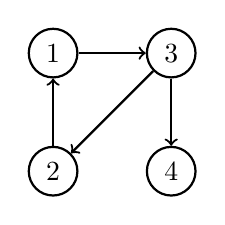
\begin{tikzpicture}[node distance={15mm}, thick, main/.style = {draw, circle}]
\node[main] (1) {$1$};
\node[main] (2) [below of=1] {$2$};
\node[main] (3) [right of=1] {$3$};
\node[main] (4) [below of=3] {$4$};
\draw[->] (1) -- (3);
\draw[->] (3) -- (4);
\draw[->] (3) -- (2);
\draw[->] (2) -- (1);
\end{tikzpicture}

using $-$ to represent $nil$, the adjacency matrix of the digraph is

$\begin{bNiceMatrix}%
 [first-col,
  first-row,
  code-for-first-col = \color{blue},
  code-for-first-row = \color{blue}]
& 1 & 2 & 3 & 4     \\
1 &  - & - & 1 & -  \\
2 &  1 & - & - &-\\
3 &  - & 1 & - & 1\\
4 &  - & - & - & -
\end{bNiceMatrix}$

An adjacency matrix, like the one above, is what is passed in to the algorithm as its last parameter.

\begin{align*}
build\_tc\ ::\ &a\ a\ [\{a,a\}\looparrowleft a]\rightarrow [\{a,a\}\looparrowleft a:::Integer]\\
build\_tc\ ::\ &0\ \_\ matrix\rightarrow matrix;\\
build\_tc\ ::\ &diagonal\_index\ size\ matrix\rightarrow\\
	&row\_indices\leftarrow \f ilter\_vector\ \{diagonal\_index,size\}\ matrix\\
	&\qquad\quad\lambda\ ::\ \{i,j\}\ matrix\rightarrow \{i,j\}\twoheadrightarrow matrix = 1\\
	&\qquad\quad\lambda\ ::\ \{i,j\}\rightarrow \{i,j-1\},\\
	&column\_indices\leftarrow \f ilter\_vector\ \{diagonal\_index,size\}\ matrix\\
	&\qquad\quad\lambda\ ::\ \{i,j\}\ matrix\rightarrow \{i,j\}\twoheadrightarrow matrix = 1\\
	&\qquad\quad\lambda\ ::\ \{i,j\}\rightarrow \{i-1,j\},\\
	&build\_tc\ diagonal\_index-1\ size\\
	&\qquad\quad(update\ row\_indices\ column\_indicies\ matrix).
\end{align*}


\subsubsection{Sub-Algorithm}
Time Complexity: $\mathcal{O}(1)$, average case $\mathcal{O}(m^2\log n)$ where $m<n$, worst case $\mathcal{O}(n^3)$. The best case is achieved when either list of vertices is initially empty. The worst case is when the both vertex lists are the height of the matrix.

\begin{align*}
update\ ::\ &[\{a,a\}]\ [\{a,a\}]\ [\{a,a\}\looparrowleft a]\rightarrow [\{a,a\}\looparrowleft a:::Integer]\\
update\ ::\ &[]\ \_\ matrix\rightarrow matrix;\\
update\ ::\ &\_\ []\ matrix\rightarrow matrix;\\
update\ ::\ &[h\mid t]\ vertices\ matrix\rightarrow\\
	&update\_for\ h\ vertices\ matrix.
\end{align*}


\subsubsection{Sub-Algorithm}
Time Complexity: best case $\mathcal{O}(1)$, average case $\mathcal{O}(m\log n)$ where $m<n$, worst case $\mathcal{O}(n^2)$. The best case occurs when the vertex list is initially empty. The worst case is when $m=n$, the length of the vertex list is the size of the matrix.
\begin{align*}
update\_for\ ::\ &\{a,a\}\ [\{a,a\}]\ [\{a,a\}\looparrowleft a]\rightarrow [\{a,a\}\looparrowleft a:::Integer]\\
update\_for\ ::\ &\_\ []\ matrix\rightarrow matrix;\\
update\_for\ ::\ &\{i,j\}\ [\{k,\ell\}\mid t]\ matrix\when k \ne j\land i\ne \ell\rightarrow\\
	&update\_for\ \{i,j\}\ t\ matrix;\\
update\_for\ ::\ &\{i,j\} [\{k,\ell\}\mid t]\ matrix\rightarrow\\
	&case\ i=\ell\\
	&\quad true\rightarrow update\_for\ \{i,j\}\ t\ (matrix\twoheadleftarrow \{k,j\}\ 1)\\
	&\quad\false\rightarrow update\_for\ \{i,j\}\ t\ (matrix\twoheadleftarrow \{i,\ell\}\ 1).
\end{align*}

\subsubsection{Co-Algorithm}
Time Complexity: $\mathcal{O}(n^2)$.

The $\f ilter\_vector$ algorithm's behavior is to filter the $i$ and $j$ index pairs of an indicated vector of the provided matrix based on the value of at the pair$\{i,j\}$. The matrix is represented by a dictionary with the keys being $\{i,j\}$ tuples and the value being any type.

The algorithm has, as parameters, two lambda algorithms. The first, $\lambda_1$ has $\lambda_1\ ::\ \{a,a\}\ [\{a,a:::Integer\}\looparrowleft b]\rightarrow Boolean$ as its signature where $b$ is of any type. $\lambda_1$'s behavior is a comparator for inclusion, $true$ indicating inclusion in the resulting list.

$\lambda_2$ has $\lambda_2\{a,a\}\rightarrow\{a,a:::Integer\}$ as its signature. Its behavior is to decrement or increment either or both of the elements of the tuple that is its parameter. I have described these two lambdas here rather than in the pseudocode to ease its reading.
\begin{align*}
\f ilter\_vector\ ::\ &\{a,a\}\ [\{a,a\}\looparrowleft a]\ \lambda_1\ \lambda_2\rightarrow [\{a,a\}]\\
\f ilter\_vector\ ::\ &\{i,j\}\ \_\ \_\ \_\when i==0 \lor j==0\rightarrow [];\\
\f ilter\_vector\ ::\ &\{i,j\}\ matrix\ \lambda_1\ \lambda_2\rightarrow\\
	&case\ \lambda_1\ \{i,j\}\ matrix\\
	&\quad \false\rightarrow vector\_filter\ (\lambda_2\ \{i,j\})\ matrix\ \lambda_1\ \lambda_2\\
	&\quad true\rightarrow [\{i,j\}]\doubleplus vector\_filter\ (\lambda_2\ \{i,j\})\ matrix\ \lambda_1\ \lambda_2.
\end{align*}

\subsection{Floyd's Algorithm}
Time Complexity: $\mathcal{O}(n^3)$ where $n$ is the size of the square matrix.

Floyd's algorithm is much like Warshall's. The main differences being 1) using a distance matrix instead of an adjacency matrix, and 2) putting a sum of distances in the matrix instead of just a $1$ when an appropriate index is found. The replacement only happens if the sum is less than the value currently stored at that index. It should, therefore, come as no surprise that the algorithms look very similar in pseudocode.

The algorithm below uses one unique sub-algorithm, and reuses the $\f ilter\_vector$ algorithm we used to implement Warshall's algorithm. I've chosen to name the algorithm in the pseudocode \textit{build s}hortest \textit{p}ath \textit{m}atrix.

\begin{align*}
build\_spm\ ::\ &a\ a\ [\{a,a\}\looparrowleft a]\rightarrow [\{a,a\}\looparrowleft a:::Integer]\\
build\_spm\ ::\ &0\ \_\ matrix\rightarrow matrix;\\
build\_spm\ ::\ &diagonal\_index\ size\ matrix\rightarrow\\
	&row\_indices\leftarrow \f ilter\_vector\ \{diagonal\_index,size\}\ matrix\\
	&\qquad\quad\lambda\ ::\ \{i,j\}\ matrix\rightarrow \{i,j\}\twoheadrightarrow matrix \ne\infty\\
	&\qquad\quad\lambda\ ::\ \{i,j\}\rightarrow \{i,j-1\},\\
	&column\_indices\leftarrow \f ilter\_vector\ \{diagonal\_index,size\}\ matrix\\
	&\qquad\quad\lambda\ ::\ \{i,j\}\ matrix\rightarrow \{i,j\}\twoheadrightarrow matrix \ne\infty\\
	&\qquad\quad\lambda\ ::\ \{i,j\}\rightarrow \{i-1,j\},\\
	&build\_spm\ diagonal\_index-1\ size\\
	&\qquad\quad(update\_distances\_for\ row\_indices\ column\_indicies\ matrix).
\end{align*}

\subsubsection{Sub-Algorithm}
Time Complexity: best case $\mathcal{O}(1)$, average case $\mathcal{O}(m^2\log n)$ where $m<n$, worst case $\mathcal{O}(n^3)$. The best case is achieved when either list of vertices is initially empty. The worst case is when the both vertex lists are the height of the matrix.

\begin{align*}
update\_distances\ ::\ &[\{a,a\}]\ [\{a,a\}]\ [\{a,a\}\looparrowleft a]\rightarrow [\{a,a\}\looparrowleft a:::Integer]\\
update\_distances\ ::\ &[]\ \_\ matrix\rightarrow matrix;\\
update\_distances\ ::\ &\_\ []\ matrix\rightarrow matrix;\\
update\_distances\ ::\ &[h\mid t]\ vertices\ matrix\rightarrow\\
	&update\_distances\_for\ h\ vertices\ matrix.
\end{align*}

\subsubsection{Sub-Algorithm}
Time Complexity: best case $\mathcal{O}(1)$, average case $\mathcal{O}(m\log n)$ where $m<n$, worst case $\mathcal{O}(n^2)$. The best case occurs when the vertex list is initially empty. The worst case is when $m=n$, the length of the vertex list is the size of the matrix.

This sub-algorithm uses the $min$ co-algorithm. It has as its value the least of its two numeric parameters.

\begin{align*}
update\_distances\_for\ ::\ &\{a,a\}\ [\{a,a\}]\ [\{a,a\}\looparrowleft a]\rightarrow [\{a,a\}\looparrowleft a:::Integer]\\
update\_distances\_for\ ::\ &\_\ []\ matrix\rightarrow matrix;\\
update\_distances\_for\ ::\ &\{i,j\}\ [\{k,\ell\}\mid t]\ matrix\when k \ne j\land i\ne \ell\rightarrow\\
	&update\ tr\ t\ matrix;\\
update\_distances\_for\ ::\ &\{i,j\}\ [\{k,\ell\}\mid t]\ matrix\rightarrow\\
	&sum\leftarrow \{i,j\}\twoheadrightarrow matrix + \{k,\ell\}\twoheadrightarrow matrix,\\
	&case\ i=\ell\\
	&\quad true\rightarrow\\
	&\qquad least\leftarrow min\ sum\ (\{k,j\}\twoheadrightarrow matrix),\\
	&\qquad update\ \{i,j\}\ t\ (matrix\twoheadleftarrow \{k,j\}\ least)\\
	&\quad\false\rightarrow\\
	&\qquad least\leftarrow min\ sum\ (\{i,\ell\}\twoheadrightarrow matrix),\\
	&\qquad update\_distances\_for\ \{i,j\}\ t\ (matrix\twoheadleftarrow \{i,\ell\}\ least).
\end{align*}

\chapter{Greedy Technique}

\section{Prim's Algorithm}
Time Complexity: $\mathcal{O}(n\log n)$ where $n$ is the number edges in the graph. There is a better, though more complicated, version of this algorithm which has a complexity of $\mathcal{O}(n\log m)$ where $m$ is the number of vertices in the graph. As the density of increases, the difference in the complexity decreases, aproaching $0$.

Prim's Algorithm produces a collection of nodes and distances that make up the Optimal Minimum Spanning Tree (OMST) of an undirected graph. The algorithm described here uses a dictionary for both the graph and the OMST. The keys for both of these trees is a node. The value for each key is a tuple consisting of the connected graph node and the distance between it and the key node. It is important to note that the undirected graph is represented by a directed graph with two edges between each pair of connected nodes.
\begin{align*}
find\_omst\ ::\ &a\ [a\looparrowleft [\{a,b\}]]\ [a]_{set}\ [\{a,a,b\}]_{min\_heap}\ [a\looparrowleft \{a,b\}]\rightarrow [a\looparrowleft \{a,b\}]\\
find\_omst\ ::\ &\_\ \_\ visited\_nodes\ []\ omst\when visited\_nodes\ne []\rightarrow omst;\\
find\_omst\ ::\ &node\ graph\ visited\_nodes\ avail\_nodes\ omst\rightarrow\\
	&\{n_1,n_2,distance\}\leftarrow get\_next\_edge\\
	&\qquad\quad(add\_to\_avail\ node\ visited\ avail\_nodes),\\
	&find\_omst\ n_1\ graph\ [n_1]\doubleplus[n_2]\doubleplus visited\\
	&\qquad\quad[\{n_1,n_2,distance\}]\doubleplus omst.
\end{align*}
\subsection{Sub-Algorithm}
Time Complexity: best case $\mathcal{O}(n)$, average and worst case $\mathcal{O}(n\log m)$ where $n$ is the number edges to add and $m$ is the number of edges already in the min-heap. 
\begin{align*}
add\_to\_avail\ ::\ &a\ [a]\ [\{a,b\}]\rightarrow[\{a,a,b\}]\\
add\_to\_avail\ ::\ &\_\ []\rightarrow[];\\
add\_to\_avail\ ::\ &node\ visited\ [\{adj\_node,dist\}\mid t]\when node\twoheadrightarrow visited = true\rightarrow\\
	&add\_to\_avail\ node\ t;\\
add\_to\_avail\ ::\ &node\ visited\ [\{adj\_node,dist\}\mid t]\rightarrow\\
	&[\{node,adj\_node,dist\}]\doubleplus add\_to\_avail\ node\ t.
\end{align*}

\subsection{Sub-Algorithm}
Time Complexity: best case $\mathcal{O}(1)$, average and worst case $\mathcal{O}(n)$. With $n$ begin the number of elements in the min-heap. The worst case occurs when there are a series of minimal edges in the min-heap all of which have already been visited.
\begin{align*}
get\_next\_edge\ ::\ &[\{a,a,b\}]_{min\_heap}\ [a]\rightarrow\{\{a,a,b\},[\{a,a,b\}]_{min\_heap}\}\\
get\_next\_edge\ ::\ &[]\ \_\rightarrow \{nil,[]\};\\
get\_next\_edge\ ::\ &[\{n_1,n_2,dist\}\mid t]\ visited\when n_1\not\in visited \land n_2\not\in visited\rightarrow\\
	&\{\{n_1,n_2,dist\}, t\};\\
get\_next\_edge\ ::\ &[h\mid t]\ visited\rightarrow\\
	&get\_next\_edge\ t\ visited.
\end{align*}

\section {Kruskal's Algorithm}
Time Complexity: $\mathcal{O}(n\log n)$ where $n$ is the number of edges sorted by weight.
\begin{align*}
build\_mst\ ::\ &a\ [\{a,a,b\}]\ [[a]_{set}]\ [\{a,a,b\}]\rightarrow [\{a,a,b\}]\\
build\_mst\ ::\ &1\ \_\ \{\_,mst\}\rightarrow mst;\\
build\_mst\ ::\ &node\_count\ [\{n_1,n_2,dist\}\mid t]\ visited\ mst\\
	&\qquad\qquad\when (is\_cyclic\ visited)\rightarrow\\
	&build\_mst\ (node\_count -1)\ t\ visited\ mst;\\
build\_mst\ ::\ &node\_count\  [\{n_1,n_2,dist\}\mid t]\ visited\ mst\rightarrow\\
	&build\_mst\ (node\_count -1)\ t\\
	&\qquad\quad(add\_or\_merge\ n_1\ n_2\ visited\ nil)\\
	&\qquad\quad([\{n_1,n_2,dist\}]\doubleplus mst).
\end{align*}
\subsection{Sub-Algorithm}
Time Complexity:$\mathcal{O}(n\log m)$ where n is the number of disjoint graphs and m is the number of nodes in the disjoint graphs.

This sub-algorithm indicates if the addition of the two nodes, indicated by their labels, would create a cycle if added to any disjoint graph in the list of disjoint graphs.

\begin{align*}
is\_cyclic\ ::\ &a\ a\ [[a]_{set}]\rightarrow Boolean\\
is\_cyclic\ ::\ &\_\ \_\ []\rightarrow \false;\\
is\_cyclic\ ::\ &\ell_1\ \ell_2\ [h\mid t]\when \ell_1,\ell_2\in h\rightarrow\\ true;\\
is\_cyclic\ ::\ &\ell_1\ \ell_2\ [\_\mid t]\rightarrow \\
	&is\_cyclic\ \ell_1\ \ell_2\ t. 
\end{align*}

\subsection{Sub-Algorithm}
Time Complexity:$\mathcal{O}(n\log m)$ where n is the number of disjoint graphs and m is the number of nodes in the disjoint graphs.

This sub-algorithm is here for completeness only. It may or not produce more light on the subject of Kruskell's algorithm therefore reading it is not necessarily in your best interest. 

The sub-algorithm tracks the sets of nodes corresponding to disjoint graphs created as the $build\_mst$ algorithm is used. This sub-algorithm consists of nothing more than dealing with a bunch of conditions that determine which disjoint graph the nodes should be added to, if a new disjoint graph should be created, or if two disjoint graphs are to be combined when one node is found in each disjoint graph.

The disjoint graphs are represented as disjoint sets of node labels.

\begin{align*}
add\_or\_merge\ ::\ &a\ a\ [[a]_{set}]\ [a]\rightarrow [[a\_{set}]]\\
add\_or\_merge\ ::\ &n_1\ n_2\ []\ nil\rightarrow\\
	&[[n_1,n_2]_{set}];\\
	add\_or\_merge\ ::\ &n_1\ n_2\ []\ node\_set\rightarrow\\
	&[node\_set\twoheadleftarrow n_1\twoheadleftarrow n_2];\\
add\_or\_merge\ ::\ &n_1\ n_2\ [h\mid t]\ \_\when n_1\in h\land n_2\in h\rightarrow\\
	&[n_1,n_2]_{set}\doubleplus h\doubleplus t;\\
add\_or\_merge\ ::\ &n_1\ n_2\ [h\mid t]\ nil\when n_1\in h\lor n_2\in h\rightarrow\\
	&add\_or\_merge\ n_1\ n_2\ t\ h;\\
add\_or\_merge\ ::\ &n_1\ n_2\ visited\ node\_set\when n_1\in h\lor n_2\in h\rightarrow\\
	&merged\leftarrow node\_set\cup h\twoheadleftarrow n_1\twoheadleftarrow\ n_2,\\
	&merged\doubleplus visited;\\
add\_or\_merge\ ::\ &n_1\ n_2\ [h\mid t]\ node\_set\rightarrow\\
	&h\doubleplus add\_or\_merge\ n_1\ n_2\ t\ node\_set.
\end{align*}

\section{Disjoint Subsets and Union-Find Algorithms}
None.
\section{Dijkstra's Algorithm}
Time Complexity: $\mathcal{O}(e\log v)$ where $e$ is the number of edges and $v$ is the number of vertices.

In the algorithm and sub-algorithms described here, the type of $a$ any comparable type. This could be a character, a string, a number, etc. The type of $b$ is any summable type. This could be an $Integer$, a $Real$, or some other type for which addition has been defined.

A min-heap, otherwise known as a priority queue, a dictionary, and a set are used in this description of Dijkstra's Algorithm. By choosing other types of data structures, other time complexities can be achieved.

When all nodes have been visited, the algorithm terminates.

\begin{align*}
find\_costs\_given\ ::\ &[a\looparrowleft [\{a,b\}]\ [\{a,b\}]_{min\_heap}\ [a]_{set}\ c:::Integer\rightarrow [\{a,b\}]\\
find\_costs\_given\ ::\ &\_\ \_\ \_\ 0\rightarrow [];\\
find\_costs\_given\ ::\ &adjacent\_costs\ heap\ visited\ counter\rightarrow\\
	&\{\{node,node\_cost\},u\_heap,upd\_visited\}\leftarrow get\_least\ heap\ visited,\\
	&[\{node,node\_cost\}]\doubleplus\\ 
	&\qquad\quad find\_costs\_given\\
	&\qquad\qquad adjacent\_costs\\
	&\qquad\qquad (add\_to\ u\_heap\ (node\twoheadrightarrow adjacent\_costs)\ node\_cost)\\
	&\qquad\qquad upd\_visited\ counter-1.
\end{align*}

\subsection{Sub-Algorithm}
Time Complexity: $\mathcal{O}(n\log m)$ where $n$ is the number of insertions to do, the edge count for a given node, and $m$ is the number of elements in the min-heap.
\begin{align*}
add\_to\ ::\ &[\{a,b\}]_{min\_heap}\ [\{a,b\}]\ b\rightarrow [\{a,b\}]_{min\_heap}\\
add\_to\ ::\ &heap\ []\ \_\rightarrow heap;\\
add\_to\ ::\ &heap\ [\{node,cost\}\mid t]\ base\_cost\rightarrow\\
	&[\{node,cost+base\_cost\}]\doubleplus add\_to\ heap\ t\ base\_cost.
\end{align*}
\subsection{Sub-Algorithm}
Time Complexity: best case $\mathcal{O}(1)$, worst and average case $\mathcal{O}(n\log n)$ where $n$ is the number of nodes already visited.
\begin{align*}
get\_least\ ::\ &[\{a,b\}]_{min\_heap}\ [a]_{set}\rightarrow \{\{a,b\},[\{a,b\}]_{min\_heap},[a]_{set}\}\\
get\_least\ ::\ &[\{node,base\_cost\}\mid t]\ visited\when node\in visited\rightarrow\\
	&get\_least\ t\ visited;\\
get\_least\ ::\ &[\{node,base\_cost\}\mid t]\ visited\rightarrow\\
	&\{\{node,base\_cost\},t,[node]\doubleplus visited\}.
\end{align*}

\chapter{Iterative Improvement}
\section{The Simplex Method}
none
\section{The Maximum-Flow Problem}

For this algorithm and its sub-algorithms, $\ell$ is any type that can be used to label a node and $a$ is any comparable, summable type.

The algorithm described here is the Edmunds-Karp algorithm for finding the max-flow through a directed graph.
\begin{align*}
calculate\_flow\ ::\ &\ell\ \ell\ [\ell\looparrowleft [\{\ell,a,a\}]\ a\rightarrow a\\
calculate\_flow\ ::\ &source\ sink\ graph\ flow\rightarrow\\
	&case\ find\_shortest\_path\ sink\ [\{source,\infty\}]\ graph,\\
	&\quad\%\%\text{If there are no more unexplored paths.}\\
	&\quad nil\rightarrow\\
	&\qquad flow\\
	&\quad\%\%\text{If there is at least one unexplored path.}\\
	&\quad\{path,path\_flow\}\rightarrow\\
	&\qquad u\_graph\leftarrow update\_used\ \{path,path\_flow\}\ graph,\\
	&\qquad calculate\_flow\ source\ sink\ u\_graph\ (flow+path\_flow).
\end{align*}
\subsection{Sub-Algorithm}

The definition of shortest path used here is the path with the fewest edges that leads from the source to the sink.
\begin{align*}
find\_shortest\_path\ ::\ &\ell\ [\{[\ell],a\}]\ [\ell\looparrowleft [\{\ell,a,a\}]\rightarrow \{[\ell],a\}\\
find\_shortest\_path\ ::\ &sink\ [\{[\ell\mid qt],bottleneck\}\mid t]\ graph\\
	&\qquad\qquad\when\\
	&\qquad\qquad(at\_end\ sink\ \ell\twoheadrightarrow graph) = \{true,s,capacity\}\rightarrow\\
	&\{[sink]\doubleplus[\ell]\doubleplus qt,(min\ capacity\ bottleneck)\};\\
find\_shortest\_path\ ::\ &sink\ [\{[\ell\mid qt],bottleneck\}\mid t]\ graph\\
	&case [\{n,c,u\}\mid \{n,c,u\}\in (\ell\twoheadrightarrow graph),c-u>0],\\
	&\quad[]\rightarrow\\
	&\qquad nil\\
	&\quad nodes\rightarrow\\
	&\qquad updated\_paths\leftarrow extend\_path\ ([\ell]\doubleplus qt)\\
	&\qquad\qquad\{nodes,bottleneck\}\\
	&\qquad\qquad find\_shortest\_path\ (t\doubleplus updated\_paths)\ graph.
\end{align*}
\subsection{Sub-Algorithm}
\begin{align*}
extend\_path\ ::\ &[\ell]\ [\{\ell,a,a\}]\ a\rightarrow [\{[\ell],a\}]\\
extend\_path\ ::\ &\_\ []\ \_\rightarrow [];\\
extend\_path\ ::\ &path\ [\{\ell,constraint,used\}\mid t]\ bottleneck\rightarrow\\
	&[\{[\ell]\doubleplus path,min\ bottleneck\ (constraint-used)\}]\\
	&\doubleplus\\
	&extend\_path\ path\ t\ bottleneck.
\end{align*}
\subsection{Sub-Algorithm}
This sub-algorithm updates each node in the path. It changes the nodes' $used$ description element by adding the additional flow through the node due to the flow for this path. This algorithm accomplishes what is often called the 'backwards' portion of the algorithm.
\begin{align*}
update\_used\ ::\ &\{[\ell],a\}\ [\ell\looparrowleft [\{\ell,a,a\}]\rightarrow [\ell\looparrowleft [\{\ell,a,a\}]\\
update\_used\ ::\ &[]\ graph\rightarrow graph;\\
update\_used\ ::\ &\{[h\mid t],path\_flow\}\ graph\rightarrow\\
	&\{\ell,capacity,used\}\leftarrow h\twoheadrightarrow graph,\\
	&update\_used\ \{t,path\_flow\}\\
	&\quad(graph\twoheadleftarrow\ h\ \{\ell,capacity,used+path\_flow\}).
\end{align*}
\subsection{Sub-Algorithm}
This sub-algorithm determines if the sink node has been found. It is here for completeness but is of little interest. Read it if it will help you understand its parent algorithm. Don't read it if it wont.
\begin{align*}
at\_end\ ::\ &\ell\ [\{\ell,a,a\}]\rightarrow Boolean\\
at\_end\ ::\ &sink\ []\rightarrow\false;\\
at\_end\ ::\ &sink\ [\{\ell,\_,\_\}\mid t]\when \ell=sink\rightarrow true;\\
at\_end\ ::\ &sink\ [h\mid t]\rightarrow\\
	&at\_end\ sink\ t.
\end{align*}
\subsection{Maximum Matching in Bipartite Graphs}

The second parameter of this algorithm is a list containing vertices from one of the halves of the graph. The first parameter is a queue of vertices from the second parameter that have no matched vertex. The third parameter is the entire graph, the fourth parameter is a working, temporary accumulator where the labeling, mentioned in the reading, is stored for later use. The last parameter is an accumulator containing the matching that eventually becomes the maximum matching. When this algorithm is used, the matching would be an empty dictionary.
\begin{align*}
maximize\ ::\ &[\ell]_{queue}\ [\ell]\ [\ell\looparrowleft\ell]\ [\ell\looparrowleft\ell]\rightarrow [\ell\looparrowleft\ell]\\
maximize\ ::\ &[]\ \_\ \_\ labels\ matching\ \rightarrow matching;\\
maximize\ ::\ &[h\mid t]\ v\_nodes\ graph\ labels\ matching\rightarrow\\
	&case\ adjust\_all\ (h\twoheadrightarrow graph)\ h\ matching\ labels\\
	&\%\%\text{the sub-algorithm terminated early}\\
	&\quad\{true,updated\_matching,\_\}\rightarrow,\\
	&\qquad free\_nodes\leftarrow [\ell\mid \ell\in v\_nodes,\ell\twoheadrightarrow updated\_matching = nil],\\
	& \qquad maximize\ free\_nodes\ graph\ updated\_matching\ [\ \looparrowleft\ ]\\
	&\%\%\text{the sub-algorithm ran through the entire list of nodes adjacent to } h\\
	&\quad\{\false,updated\_matching,updated\_labels\}\rightarrow\\
	&\qquad\ maximize\ t\ v\_nodes\ graph\ updated\_matching\ updated\_labels.
\end{align*}
\subsection{Sub-Algorithm}

This sub-algorithm selects, labels, and adds to the matching nodes that are adjacent to the second parameter that are not yet labeled.
\begin{align*}
adjust\_all\ ::\ &[\ell]\ \ell\ [\ell\looparrowleft\ell]\ [\ell\looparrowleft\ell]\ [\ell]\rightarrow\{Boolean,[\ell\looparrowleft\ell]\ [\ell\looparrowleft\ell]\}\\
adjust\_all\ ::\ &[]\_\ matching\ labels\ \_\rightarrow\{\false,matching,labels\};\\
adjust\_all\ ::\ &[h\mid \_]\ node\ matching\ labels\ \_\when\\
	&\qquad\quad(node\twoheadrightarrow matching = h)\lor (h\twoheadrightarrow labels\ne nil)\rightarrow\\
	&\%\%\text{ terminate early and try a different node and its adjacent nodes}\\
	&\{true,\\
	&\ changed\leftarrow update\_matching\ node\ (matching\twoheadleftarrow node\ h)\ labels,\\
	&\ labels\};\\
adjust\_all\ ::\ &[h\mid t]\ node\ matching\ labels\ queue\rightarrow\\
	&adjust\_all\ t\ node\ matching\ (labels\twoheadleftarrow h\ node)\ [h]\doubleplus queue.
\end{align*}

\subsection{Sub-Algorithm}
\begin{align*}
update\_matching\ ::\ &\ell\ [\ell\looparrowleft\ell]\ [\ell\looparrowleft\ell]\rightarrow [\ell\looparrowleft\ell]\\
update\_matching\ ::\ & vertex\ matching\ labels\when vertex\twoheadrightarrow labels=nil\rightarrow\\
	&matching;\\
update\_matching\ ::\ &vertex\ matching\ labels\rightarrow\\
	&u\leftarrow vertex\twoheadrightarrow labels,\\
	&v\leftarrow vertex\_next\twoheadrightarrow labels,\\
	&\%\%\text{remove the old match and replace it with a new one}\\
	&update\_matching\ v\ ((matching\twoheadleftarrow vertex\ nil)\twoheadleftarrow v\ u).
\end{align*}
\chapter{Limitations of Algorithm Power}
\section{Lower-Bound Arguments}
None
\section{Decision Trees}
None
\section{P, NP, and NP-Complete Problems}
None
\section{Challenges of Numerical Algorithms}
None
\end{document}